% Template for SE Project software documentation
% (c) Farhad Mehta 2021

\documentclass[11pt, oneside, a4paper]{book}

% File containing the commands and definitions
% that are used throughout this project.

% Set input encoding
\usepackage[utf8]{inputenc}

% For creating coloured text and backgrounds
\usepackage[table,xcdraw]{xcolor}

% For creating compact lists
\usepackage{paralist}

% To get the current date and time
\usepackage{datetime2}

% For including graphics
\usepackage{graphicx}

% For table positioning
\usepackage{float}

% For glossaries
\usepackage[nonumberlist]{glossaries}
\usepackage[automake, toc]{glossaries-extra}

% For table scaling
\usepackage{array}

% For multipage table
\usepackage{longtable}

% Custom commands

\newcommand{\todo}[1]{TODO: {#1}}

% The following command indicates that its content consists of instructions
% Even if it does not do anything, it is still a good idea to keep instructions within the `instruction` tag to separate them from the rest of the text. One could then typeset them differently, or choose to remove them form the document by redefining the command definition 
\newcommand{\instructions}[1]{#1}

% Uncomment the following command to remove all instructions
% \newcommand{\instructions}[1]{}

% Uncomment the following to make instructions appear in coloured boxes
% Note: The changes within `\instruction` are not visible in latexdiff when they are typeset in this way
% \usepackage{tcolorbox}
% \newcommand{\instructions}[1]{
%     \begin{tcolorbox}[sharp corners, colback=green!30, colframe=green!80!blue, title=Instructions]
%         #1
%     \end{tcolorbox}
% }

% Uncomment the following to make instructions appear in colour.
% Note: The changes within `\instructions` are not visible in latexdiff when they are typeset in this way
% \newcommand{\instructions}[1]{ { \color{blue} #1 } }

% Get a git version description roughly using the idea in  
% https://blog.wxm.be/2013/08/20/automated-git-commit-number-in-latex.html
% Note that the file that is included needs to be generated before the document is built.
% Refer to the makefile for further details.
\IfFileExists{../gitDescription.tmp}
{\newcommand{\gitDescription}{\input{../gitDescription.tmp}}}
{\newcommand{\gitDescription}{Not available}}

% Note: Importing hyperref must be done towards the end since it
% redefines many macros
%
% Note:
%  The following packages must be imported *before* hyperref:
%  
%  The following packages must be imported *after* hyperref:
%    amsrefs, geometry
\usepackage{hyperref}

\usepackage{geometry}

% options for package geometry (influences writable area on page)
% \geometry{a4paper, top=2cm, bottom=2cm}


\makeglossaries

\newglossaryentry{jass}
{
  name={Jass},
  description={A Swiss card game, see \href{https://en.wikipedia.org/wiki/Jass}{Wikipedia} for more details}
}

\newglossaryentry{coiffeur-jass}
{
  name={Coiffeur Jass},
  description={A variant of Jass which is played by four players.
  Two teams of two players each compete against each other, trying to get the higher score}
}

\newglossaryentry{trump}
{
  name={Trump},
  description={A suit can be declared as the trump suit (Trumpf), which changes the card values within that suit for the round}
}

\newglossaryentry{swiss-suited-cards}
{
  name={Swiss-suited playing cards},
  description={A big part of swiss german speaking switzerland uses the \href{https://en.wikipedia.org/wiki/Swiss-suited_playing_cards}{Swiss-suited playing cards}.
  There are four suits: \gls{bells} (Schellen), \gls{shields} (Schilten), \gls{roses} (Rosen), \gls{acorns} (Eicheln)}
}

\newglossaryentry{acorns} { name={Acorns}, description={A suit in the Swiss playing cards, also known as Eicheln} }
\newglossaryentry{roses} { name={Roses}, description={A suit in the Swiss playing cards, also known as Rosen} }
\newglossaryentry{shields} { name={Shields}, description={A suit in the Swiss playing cards, also known as Schilten} }
\newglossaryentry{bells} { name={Bells}, description={A suit in the Swiss playing cards, also known as Schellen} }

\newglossaryentry{tops-down}{
    name={Tops-down},
    description={A kind of \gls{contract} in the \gls{coiffeur-jass} which plays without a trump.
    The highest card always wins, the 8 card counts as 8 points}
}

\newglossaryentry{bottoms-up}{
    name={Bottoms-up},
    description={A kind of \gls{contract} in the \gls{coiffeur-jass} which plays without a trump.
    The lowest card always wins, the 8 card counts as 8 points and the 6 is worth 11 points, but the ace is worthless}
}

\newglossaryentry{slalom}{
    name={Slalom},
    description={A kind of \gls{contract} in the \gls{coiffeur-jass} which plays without a trump.
    Alternates between \gls{bottoms-up} and \gls{tops-down} or vice-versa, scoring rules apply from the first chosen option}
}

\newglossaryentry{guschti}{
    name={Guschti},
    description={A kind of \gls{contract} in the \gls{coiffeur-jass} which plays without a trump.
    Starts with either \gls{bottoms-up} or \gls{tops-down} for the first 5 \glspl{trick} and then flips, scoring rules apply from the first chosen option}
}

\newglossaryentry{contract}{
    name={Contract},
    description={A available option within a coiffeur.
    Possible contracts: any \gls{trump}, \gls{bottoms-up}, \gls{tops-down}, \gls{slalom} and \gls{guschti}}
}

\newglossaryentry{scoreboard}{
    name={Scoreboard},
    description={The board on which the scores (points) are tracked.
    Knows as ``Jasstafel'' in swiss german}
}

\newglossaryentry{joker}{
    name={Joker},
    description={A special \gls{contract} which can be used to do any other valid contract, even if already used}
}

\newglossaryentry{pass}{
    name={pass},
    description={A player has the option to not choose a \gls{contract} but instead pass on the decision to the next player (Schiebe).
    This can only be done once per round}
}

\newglossaryentry{trick}{
    name={Trick},
    description={A trick consists of four cards played in counter-clockwise order}
}

\newglossaryentry{round}{
    name={Round},
    description={A round starts by being dealt 9 cards and is done once all cards are played}
}

\newglossaryentry{game}{
    name={Game},
    description={A game starts by selecting the appropriate table and starting a new game.
    A game consists of 20 rounds in total, 10 for each team}
}

\newglossaryentry{score}{
    name={score},
    description={To take a \gls{trick}.
    After every player played one card from his hand the player with the strongest card in the current \gls{contract} scores}
}

\newglossaryentry{jass-table}{
    name={Jass table},
    description={Physically \gls{jass} is usually played sitting around a table.
    In \gls{coiffeur-jass}, diagonally opposite players are in the same team}
}


\hypersetup{
    pdfauthor={Pascal Honegger, Marcel Joss, David Kalchofner, Jamie Maier},
    pdftitle={JassTracker Project Documentation},
}

\begin{document}

\pagestyle{empty}

\frontmatter

\begin{titlepage}

    \begin{center}

        \vspace{1 cm}

        {\Large SE Project \\ Documentation} \\

        \vspace{0.5cm}

        {\Huge JassTracker}

        \vspace{0.5cm}

        Semester: Spring 2022

        \vspace{1 cm}

        
\includegraphics[height=5cm]{resources/se-project-logo}

        \vspace{1 cm}

        Version: 1.0 \\
        Date: \DTMnow \\
        \vspace{1 cm}

        \begin{tabular}{rl}
            \textbf{Project Team:}    & Pascal Honegger \\
                                      & Marcel Joss \\
                                      & David Kalchofner \\
                                      & Jamie Maier \\
                                      &                    \\
            \textbf{Project Advisor:} & Thomas Kälin
        \end{tabular}

        \vfill

        % 
\includegraphics[height=2cm]{resources/ost-logo.png}\\

        \vspace{1cm}
        School of Computer Science\\
        OST Eastern Switzerland University of Applied Sciences

    \end{center}

\end{titlepage}

\tableofcontents

\mainmatter


\part{Management Summary}
\chapter*{Management Summary}

\instructions{
    Even though this is the first chapter of your document, it is typically the last one filled with content. The \textit{Management Summary} is a \textbf{brief and high-level summary} of your project. It should give any reader unfamiliar to the project an overview of the contents included later in the document.
    
    \bigskip
    
    A common structure is:
    
    \begin{itemize}
        \item What is the problem we wanted to solve?
        \item How did we solve the problem?
        \item Does your solution solve the problem in a successful way?
        \item Will there be consecutive projects based on your work?
    \end{itemize}
    
    Diagrams and images work very well in this chapter, especially screenshots of your software.
    
    \bigskip
    
    One final remark: a well written management summary is a good starting point for your \textbf{Project Presentation}, as you will address a similar audience there.
}



\part{Product Documentation}
\chapter{Vision}

JassTracker is a webapp which allows tracking and analysis of the popular swiss card game \gls{jass}.
There are many different forms of playing, but the one we're focusing on is called "Coiffeur".
The following paragraphs expect the reader to know the basic rules and concepts of a "Coiffeur Jass".

\section*{What It Does}
The goal of the JassTracker is to allow the players to focus on the game without having to worry about tracking points or whose turn it is.
Instead of having to write down the scores using pen and paper, you can simply input them into the JassTracker digitally.
The website automagically tracks whose turn it is and analyses your scores for you.
You can also gain exhaustive insight into your playstyle by looking at personal or group statistics, such as average score by player or historic averages.
The system is also very flexible and can be configured to your liking.
For example, once you have configured a Jass table, you can easily start a new game with the same players.

\section*{How It Works}
The fist step is to create a new table and enter all team members for the game.
Then you start playing the game physically, just like you would normally.
Once a round is over, you input the score for the scoring member and "Trumpf".
After entering the points, a few things happen automatically:
\begin{itemize}
    \item Player \& team score update
    \item The upcoming starting person is shown
    \item Statistics refresh with latest information
\end{itemize}
When the game has finished, highlights of the game (e.g. the best player or highest round score) are displayed.

\section*{Extensions}
Some potential ideas to expand on:
\begin{itemize}
    \item Configurable Jass game (e.g. Coiffeur with 8 instead of 10 options)
    \item Prediction of scores based on historic performance
    \item Current game trajectory (win probability by team)
    \item Share the scoreboard in real time with other members, in case you want to show the scoreboard on a different device as well
    \item Associate game to personal account to track personal statistics accross games
    \item In depth statistics like playstyle, favorite "Trumpf", best "partner" by win probability etc.
    \item Charts in game to show statistics
\end{itemize}

\chapter{Requirements}

\section{Use-Case Diagram}
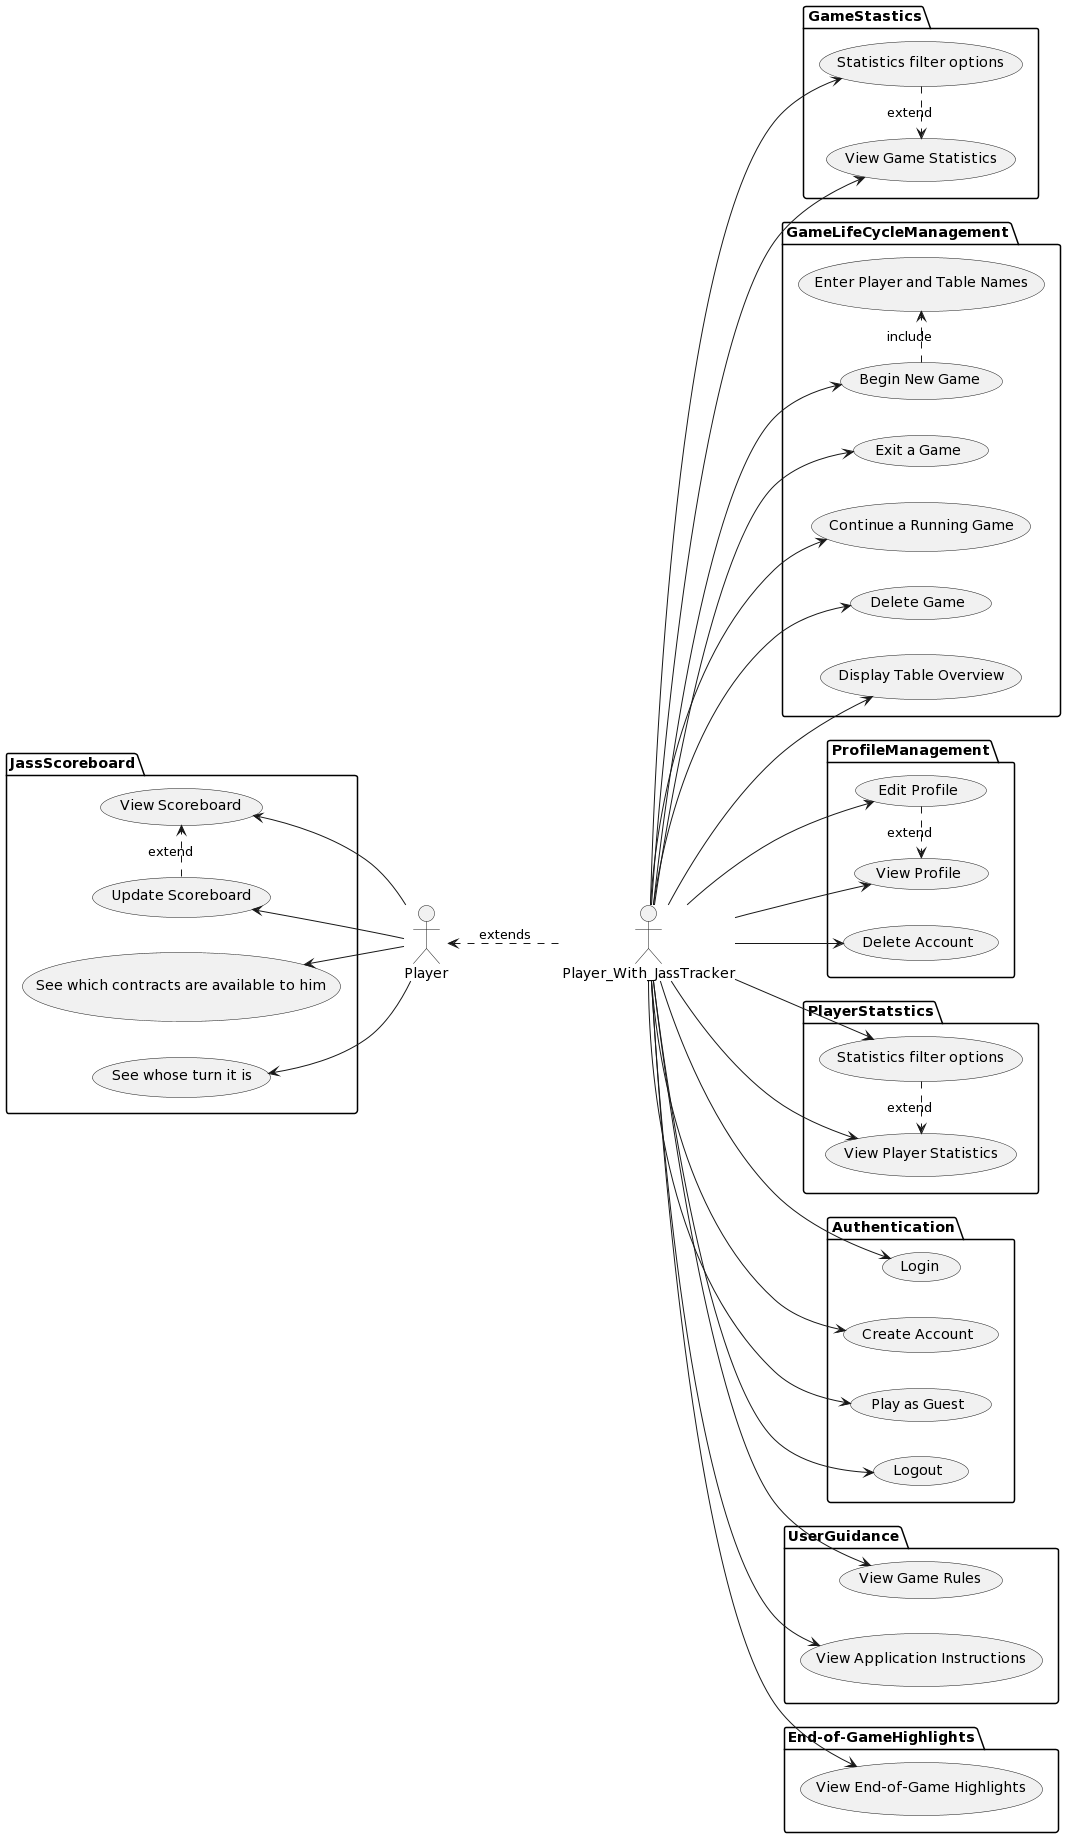
\includegraphics[height=18cm]{resources/diagrams/use-case}

\newcolumntype{s}{>{\columncolor[HTML]{c2c2cc}} m{3cm}} 

\section {Functional Requirements}

\paragraph{Info:}
The following requirements are by no means complete, but cover all key-requirements to aid the enhancement of use-cases and UI mockups. 
Also note that these requirements are not prioritized.

\subsection {Game Life Cycle Management}

\begin{tabular} { | m{1.75 cm} | m{5.25cm} | }
    \hline
    \multicolumn{1}{|c|}{\textbf{ID}} & \multicolumn{1}{|c|}{ \textbf{Story} }  \\
    \hline
    \href{https://jasstracker-jira.atlassian.net/browse/JASS-39}{JASS-39}  & New Table \& New Game Creation \\
    \hline
    \href{https://jasstracker-jira.atlassian.net/browse/JASS-43}{JASS-43} & Exit Game \\
    \hline
    \href{https://jasstracker-jira.atlassian.net/browse/JASS-41}{JASS-41} & Display Table Overview \\ 
    \hline
    \href{https://jasstracker-jira.atlassian.net/browse/JASS-42}{JASS-42} & Running \& Completed Game Distinction \\
    \hline
    \href{https://jasstracker-jira.atlassian.net/browse/JASS-41}{JASS-41} & Game Continuation \\ 
    \hline
    \href{https://jasstracker-jira.atlassian.net/browse/JASS-44}{JASS-44} & Delete Table \& Games \\
    \hline
\end{tabular}

\subsection{Jass Scoreboard}
\begin{tabular} { | m{1.75 cm} | m{5.25cm} | }
    \hline
    \multicolumn{1}{|c|}{\textbf{ID}} & \multicolumn{1}{|c|}{ \textbf{Story} }  \\
    \hline
    \href{https://jasstracker-jira.atlassian.net/browse/JASS-45}{JASS-45} & Display Current Score \\
    \hline
    \href{https://jasstracker-jira.atlassian.net/browse/JASS-47}{JASS-47} & Update Scoreboard \\
    \hline
    \href{https://jasstracker-jira.atlassian.net/browse/JASS-65}{JASS-65} & (Extension) View Win Probability per Team \\
    \hline
    \href{https://jasstracker-jira.atlassian.net/browse/JASS-64}{JASS-64} & (Extension) Display Score Prediction \\
    \hline
    \href{https://jasstracker-jira.atlassian.net/browse/JASS-66}{JASS-66} & (Extension) Share Scoreboard \\
    \hline
    \href{https://jasstracker-jira.atlassian.net/browse/JASS-48}{JASS-48} & Display Whose Turn it is \\
    \hline
    \href{https://jasstracker-jira.atlassian.net/browse/JASS-85}{JASS-85} & Display Available Contracts \\
    \hline
\end{tabular}

\subsection{Game Statistics}
\begin{tabular} { | m{1.75 cm} | m{5.25cm} | }
    \hline
    \multicolumn{1}{|c|}{ \textbf{ID}} & \multicolumn{1}{|c|}{ \textbf{Story} }  \\
    \hline
    \href{https://jasstracker-jira.atlassian.net/browse/JASS-52}{JASS-52} & Display Statistics of one Game \\
    \hline
    \href{https://jasstracker-jira.atlassian.net/browse/JASS-53}{JASS-53} & (Extension) Display comparison of two game statistics \\
    \hline
    \href{https://jasstracker-jira.atlassian.net/browse/JASS-54}{JASS-54} & Statistics filter options \\
    \hline
\end{tabular}

\subsection{Authentication}
\begin{tabular} { | m{1.75 cm} | m{5.25cm} | }
    \hline
    \multicolumn{1}{|c|}{ \textbf{ID}} & \multicolumn{1}{|c|}{ \textbf{Story} }  \\
    \hline
    \href{https://jasstracker-jira.atlassian.net/browse/JASS-51}{JASS-51} & Play as Guest \\
    \hline
    \href{https://jasstracker-jira.atlassian.net/browse/JASS-38}{JASS-38} & Account creation \\
    \hline
    \href{https://jasstracker-jira.atlassian.net/browse/JASS-37}{JASS-37} & Login \\
    \hline
    \href{https://jasstracker-jira.atlassian.net/browse/JASS-50}{JASS-50} & Logout \\
    \hline
\end{tabular}

\subsection{User Guidance}
\begin{tabular} { | m{1.75 cm} | m{5.25cm} | }
    \hline
    \multicolumn{1}{|c|}{ \textbf{ID}} & \multicolumn{1}{|c|}{ \textbf{Story} }  \\
    \hline
    \href{https://jasstracker-jira.atlassian.net/browse/JASS-36}{JASS-36} & Provide the rules of the game \\
    \hline
    \href{https://jasstracker-jira.atlassian.net/browse/JASS-56}{JASS-56} & Application Instructions \\
    \hline
\end{tabular}

\subsection{Profile Management}
\begin{tabular} { | m{1.75 cm} | m{5.25cm} | }
    \hline
    \multicolumn{1}{|c|}{ \textbf{ID}} & \multicolumn{1}{|c|}{ \textbf{Story} }  \\
    \hline
    \href{https://jasstracker-jira.atlassian.net/browse/JASS-84}{JASS-84} & Display Player Profile \\
    \hline
    \href{https://jasstracker-jira.atlassian.net/browse/JASS-33}{JASS-33} & Change Password \\
    \hline
    \href{https://jasstracker-jira.atlassian.net/browse/JASS-34}{JASS-34} & Account deletion \\
    \hline
    \href{https://jasstracker-jira.atlassian.net/browse/JASS-67}{JASS-67} & Add Display Name \\
    \hline
\end{tabular}

\subsection{Player Statistics}
\begin{tabular} { | m{1.75 cm} | m{5.25cm} | }
    \hline
    \multicolumn{1}{|c|}{ \textbf{ID}} & \multicolumn{1}{|c|}{ \textbf{Story} }  \\
    \hline
    \href{https://jasstracker-jira.atlassian.net/browse/JASS-32}{JASS-32} & Display unique player statistics \\
    \hline
    \href{https://jasstracker-jira.atlassian.net/browse/JASS-83}{JASS-83} & Statistics filter options \\
    \hline
\end{tabular}

\subsection{End-of-Game Highlights}
\begin{tabular} { | m{1.75 cm} | m{5.25cm} | }
    \hline
    \multicolumn{1}{|c|}{ \textbf{ID}} & \multicolumn{1}{|c|}{ \textbf{Story} } \\
    \hline
    \href{https://jasstracker-jira.atlassian.net/browse/JASS-68}{JASS-68} & End-of-Game Highlights \\
    \hline
\end{tabular}

\section {Non-Functional Requirements}\label{sec:NFR}

\renewcommand{\arraystretch}{1.5}

\subsection{Performance}
\begin{tabular} { |s| m{10.5cm } | }
    \hline
    \textbf{ID} & NFR-1 \\
    \hline
    \textbf{Requirement} & Reasonable response time for the rendering of new scores \\
    \hline
    \textbf{Trigger(s)} & User doesn't want to wait to see scores \\
    \hline
    \textbf{Measure(s)} & Rendering of the new scores must be doable within 1 second\\
    \hline
    \textbf{Testing} & Manual\\
    \hline
\end{tabular}
\newline
\vspace*{0.5 cm}
\newline
\begin{tabular} { |s|m{10.5cm} | }
    \hline
    \textbf{ID} & NFR-2 \\
    \hline
    \textbf{Requirement} & Authentication Response Time\\
    \hline
    \textbf{Trigger(s)} & User wants to be able to login in a timely manner\\
    \hline
    \textbf{Measure(s)} & Authentication of a user at login must be doable within 1 second\\
    \hline
    \textbf{Testing} & Manual\\
    \hline
\end{tabular}
\newline
\vspace*{0.5 cm}
\newline
\begin{tabular} { |s|m{10.5cm} | }
    \hline
    \textbf{ID} & NFR-3 \\
    \hline
    \textbf{Requirement} & New Game Creation Time\\
    \hline
    \textbf{Trigger(s)} & User wants to start the game as soon as possible\\
    \hline
    \textbf{Measure(s)} & Setting up a new game must be doable within 1 second\\
    \hline
    \textbf{Testing} & Manual\\
    \hline
\end{tabular}

\subsection{Usability}
\begin{tabular} { |s|m{10.5cm} | }
    \hline
    \textbf{ID} & NFR-4 \\
    \hline
    \textbf{Requirement} & Keyboard-only usability\\
    \hline
    \textbf{Trigger(s)} & User has no touch-screen or pointing device available\\ 
    \hline
    \textbf{Measure(s)} & Application must be usable with only a keyboard \\
    \hline
    \textbf{Testing} & Manual\\
    \hline
\end{tabular}
\newline
\vspace*{0.5 cm}
\newline
\begin{tabular} { |s|m{10.5cm} | }
    \hline
    \textbf{ID} & NFR-5 \\
    \hline
    \textbf{Requirement} & General Usability\\
    \hline
    \textbf{Trigger(s)} & Users want to be able to use the application without getting stuck\\
    \hline
    \textbf{Measure(s)} & Hallway testing shows eight people used the app without getting stuck\\
    \hline
    \textbf{Testing} & Manual\\
    \hline
\end{tabular}
\newline
\vspace*{0.5 cm}
\newline
\begin{tabular} { |s|m{10.5cm} | }
    \hline
    \textbf{ID} & NFR-6 \\
    \hline
    \textbf{Requirement} & User Guidance\\
    \hline
    \textbf{Trigger(s)} & User wants to be able to access a Help-Center\\
    \hline
    \textbf{Measure(s)} & Hallway testing shows eight people find the Help-Center and say it's helpful\\
    \hline
    \textbf{Testing} & Manual\\
    \hline
\end{tabular}


\subsection{Compatibility}
\begin{tabular} { |s|m{10.5cm} | }
    \hline
    \textbf{ID} & NFR-7 \\
    \hline
    \textbf{Requirement} & Browser Support\\
    \hline
    \textbf{Trigger(s)} & User wants to use a specific browser\\
    \hline
    \textbf{Measure(s)} & Last 2 major version of any browser with more than 1\% usage (except IE 11) is supported\\
    \hline
    \textbf{Testing} & Manual\\
    \hline
\end{tabular}
\newline
\vspace*{0.5 cm}
\newline
\begin{tabular} { |s|m{10.5cm} | }
    \hline
    \textbf{ID} & NFR-8 \\
    \hline
    \textbf{Requirement} & Mobile Device Support\\
    \hline
    \textbf{Trigger(s)} & User wants to access application using a phone or tablet\\
    \hline
    \textbf{Measure(s)} & The application must support being used on mobile devices\\
    \hline
    \textbf{Testing} & Manual\\
    \hline
\end{tabular}
\newline
\vspace*{0.5 cm}
\newline
\begin{tabular} { |s|m{10.5cm} | }
    \hline
    \textbf{ID} & NFR-18 \\
    \hline
    \textbf{Requirement} & Unicode Support\\
    \hline
    \textbf{Trigger(s)} & User wants to include special characters or emojis in his username\\
    \hline
    \textbf{Measure(s)} & Support umlauts and emojis by using utf-8 and unicode\\
    \hline
    \textbf{Testing} & Manual\\
    \hline
\end{tabular}

\subsection{Capacity}
\begin{tabular} { |s|m{10.5cm} | }
    \hline
    \textbf{ID} & NFR-9 \\
    \hline
    \textbf{Requirement} & Multiple accounts can be created \\
    \hline
    \textbf{Trigger(s)} & More than one person wants to use the application not as a guest\\
    \hline
    \textbf{Measure(s)} & At least 500 users can create an account\\
    \hline
    \textbf{Testing} & Automated\\
    \hline
\end{tabular}
\newline
\vspace*{0.5 cm}
\newline
\begin{tabular} { |s|m{10.5cm} | }
    \hline
    \textbf{ID} & NFR-10 \\
    \hline
    \textbf{Requirement} & Multiple games can be running at one time\\
    \hline
    \textbf{Trigger(s)} & A user is active in more than one game\\
    \hline
    \textbf{Measure(s)} & At least 4 games can be running at one time for a single user \\
    \hline
    \textbf{Testing} & Automated\\
    \hline
\end{tabular}

\subsection{Availability}
\begin{tabular} { |s|m{10.5cm} | }
    \hline
    \textbf{ID} & NFR-11 \\
    \hline
    \textbf{Requirement} & The application must be available \\
    \hline
    \textbf{Trigger(s)} & Application crash\\
    \hline
    \textbf{Measure(s)} & Average downtime can not exceed 30 minutes per day\\
    \hline
    \textbf{Testing} & Automated\\
    \hline
\end{tabular}

\subsection{Recoverability}
\begin{tabular} { |s|m{10.5cm} | }
    \hline
    \textbf{ID} & NFR-12 \\
    \hline
    \textbf{Requirement} & The application must not lose state \\
    \hline
    \textbf{Trigger(s)} & Application crash\\
    \hline
    \textbf{Measure(s)} & The state before crash must be recoverable\\
    \hline
    \textbf{Testing} & Automated\\
    \hline
\end{tabular}

\subsection{Maintainability}
\begin{tabular} { |s|m{10.5cm} | }
    \hline
    \textbf{ID} & NFR-13 \\
    \hline
    \textbf{Requirement} & Code Base Understanding\\
    \hline
    \textbf{Trigger(s)} & Any developer wants to be able to understand the code base\\
    \hline
    \textbf{Measure(s)} & Qodana \\
    \hline
    \textbf{Testing} & Automated\\
    \hline
\end{tabular}
\newline
\vspace*{0.5 cm}
\newline
\begin{tabular} { |s|m{10.5cm} | }
    \hline
    \textbf{ID} & NFR-14 \\
    \hline
    \textbf{Requirement} & Test-Coverage\\
    \hline
    \textbf{Trigger(s)} & User wants accountability for business functionality\\
    \hline
    \textbf{Measure(s)} & At least 80\% test-coverage is required for business logic\\
    \hline
    \textbf{Testing} & Automated\\
    \hline
\end{tabular}
\newline
\vspace*{0.5 cm}
\newline
\begin{tabular} { |s|m{10.5cm} | }
    \hline
    \textbf{ID} & NFR-15 \\
    \hline
    \textbf{Requirement} & Logging\\
    \hline
    \textbf{Trigger(s)} & User action needs to be reviewed\\
    \hline
    \textbf{Measure(s)} & At least one human readable log statement is available for each user action\\
    \hline
    \textbf{Testing} & Manual\\
    \hline
\end{tabular}
\newline
\vspace*{0.5 cm}
\newline
\begin{tabular} { |s|m{10.5cm} | }
    \hline
    \textbf{ID} & NFR-16 \\
    \hline
    \textbf{Requirement} & Lighthouse categories are acceptable\\
    \hline
    \textbf{Trigger(s)} & Users want a fast and accessible app  \\
    \hline
    \textbf{Measure(s)} & Web app should pass performance, accessibility and best practices in lighthouse with a green color (90+)\\
    \hline
    \textbf{Testing} & Automated with Gitlab CI/CD\\
    \hline
\end{tabular}

\subsection{Security}
\begin{tabular} { |s|m{10.5cm} | }
    \hline
    \textbf{ID} & NFR-17 \\
    \hline
    \textbf{Requirement} & Passwords must be secure \\
    \hline
    \textbf{Trigger(s)} & A not safe (in length) password is created\\
    \hline
    \textbf{Measure(s)} & Passwords must be at least eight characters in length\\
    \hline
    \textbf{Testing} & Automated\\
    \hline
\end{tabular}

\pagebreak
\section {Mock-ups}

\paragraph{Disclaimer:}
These are just Mock-ups.
Design can still change and colors aren't fixed and are just as a visual aid for where containers should go.


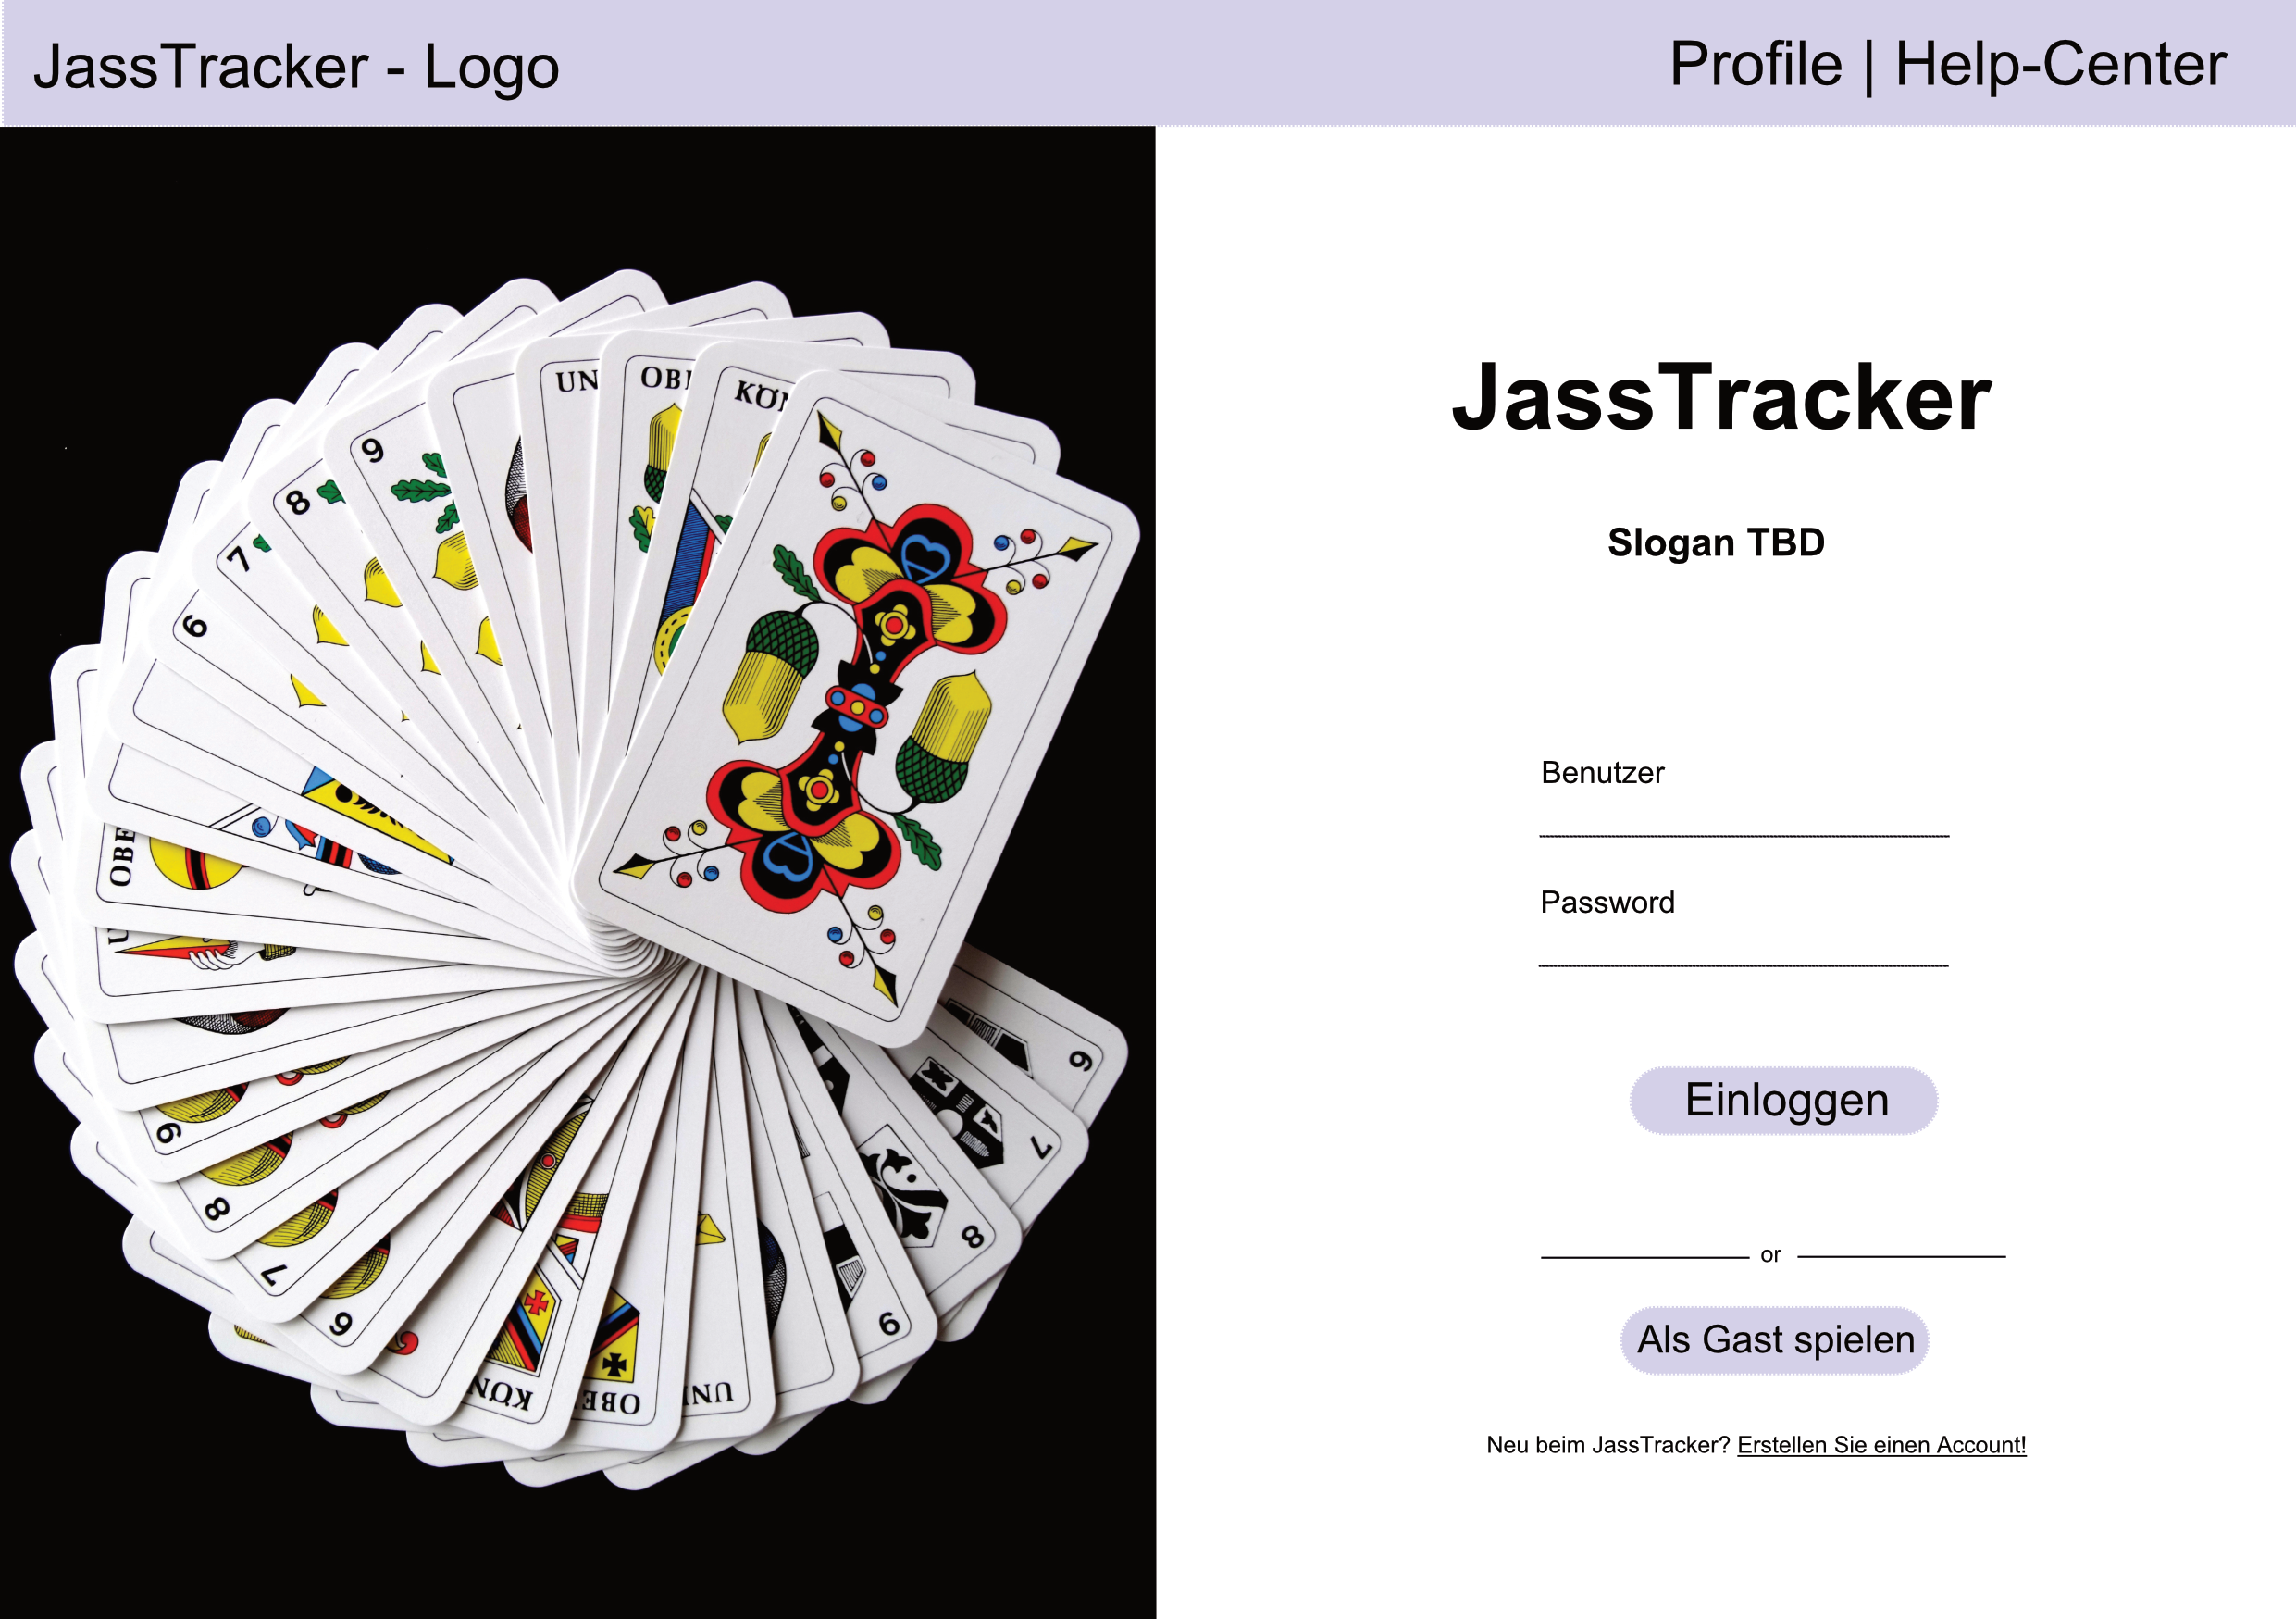
\includegraphics[height=10cm, width=\textwidth]{resources/mockups/mockup-login}
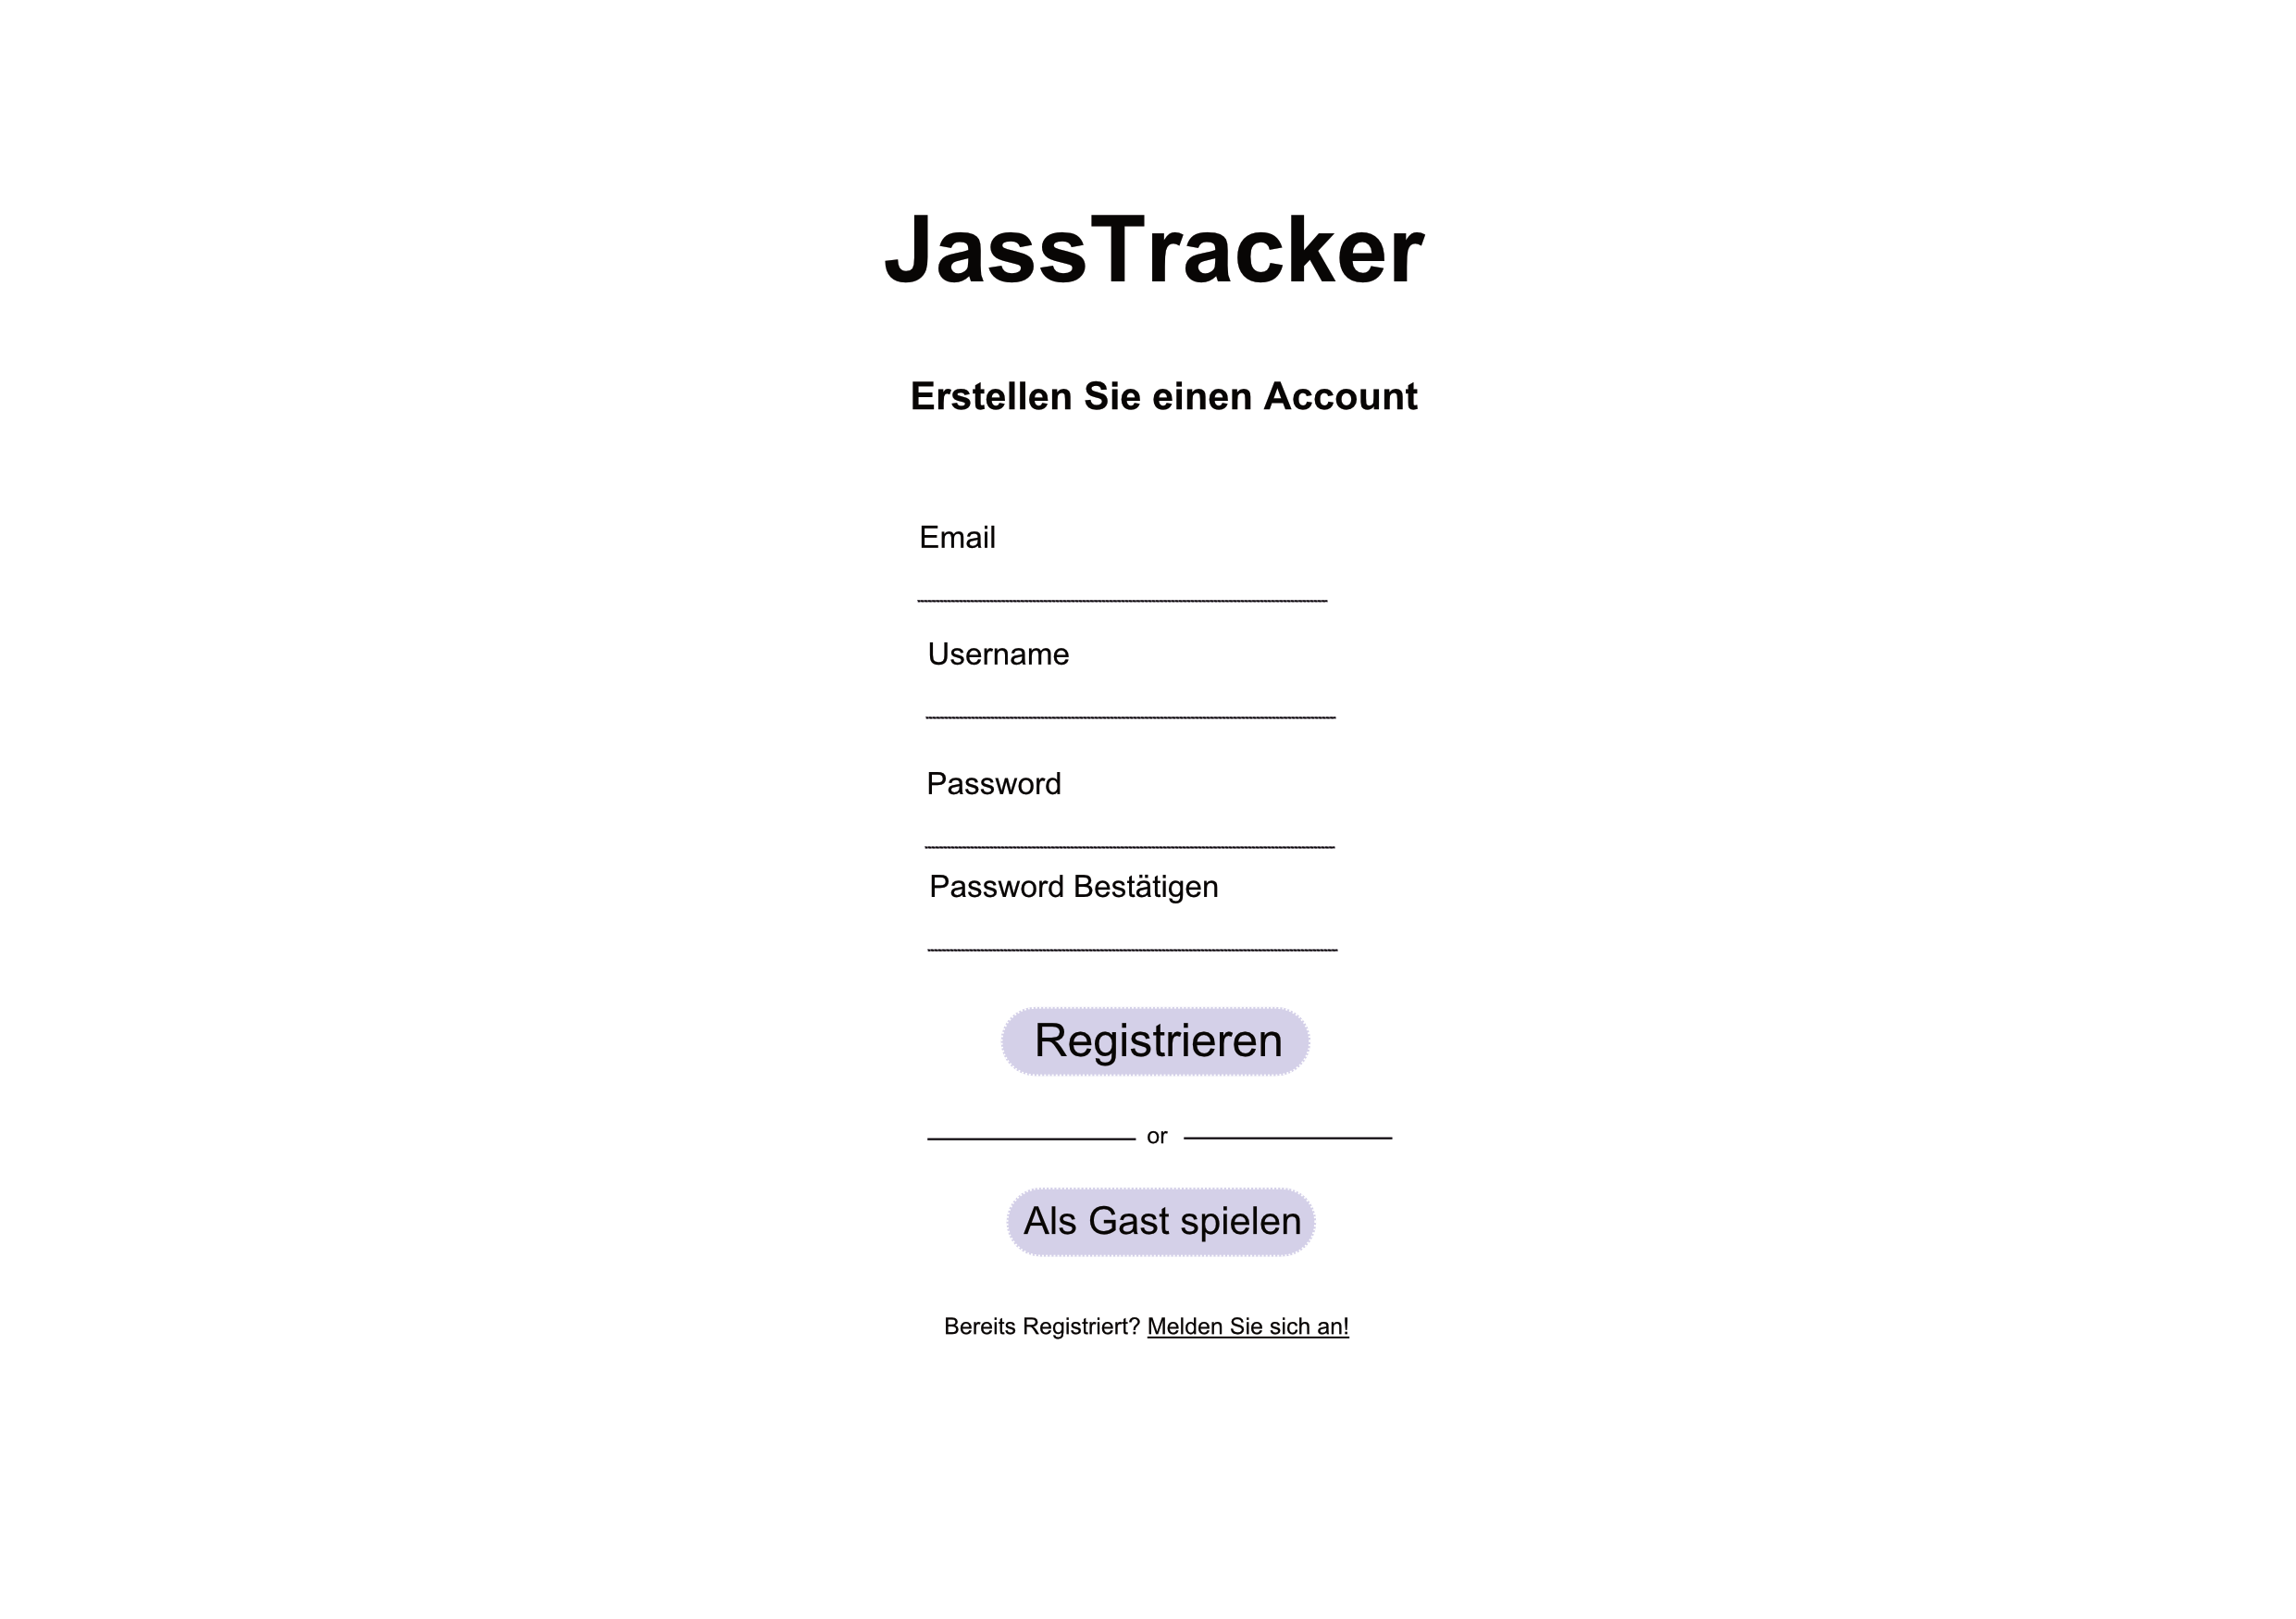
\includegraphics[height=10cm, width=\textwidth]{resources/mockups/mockup-register}
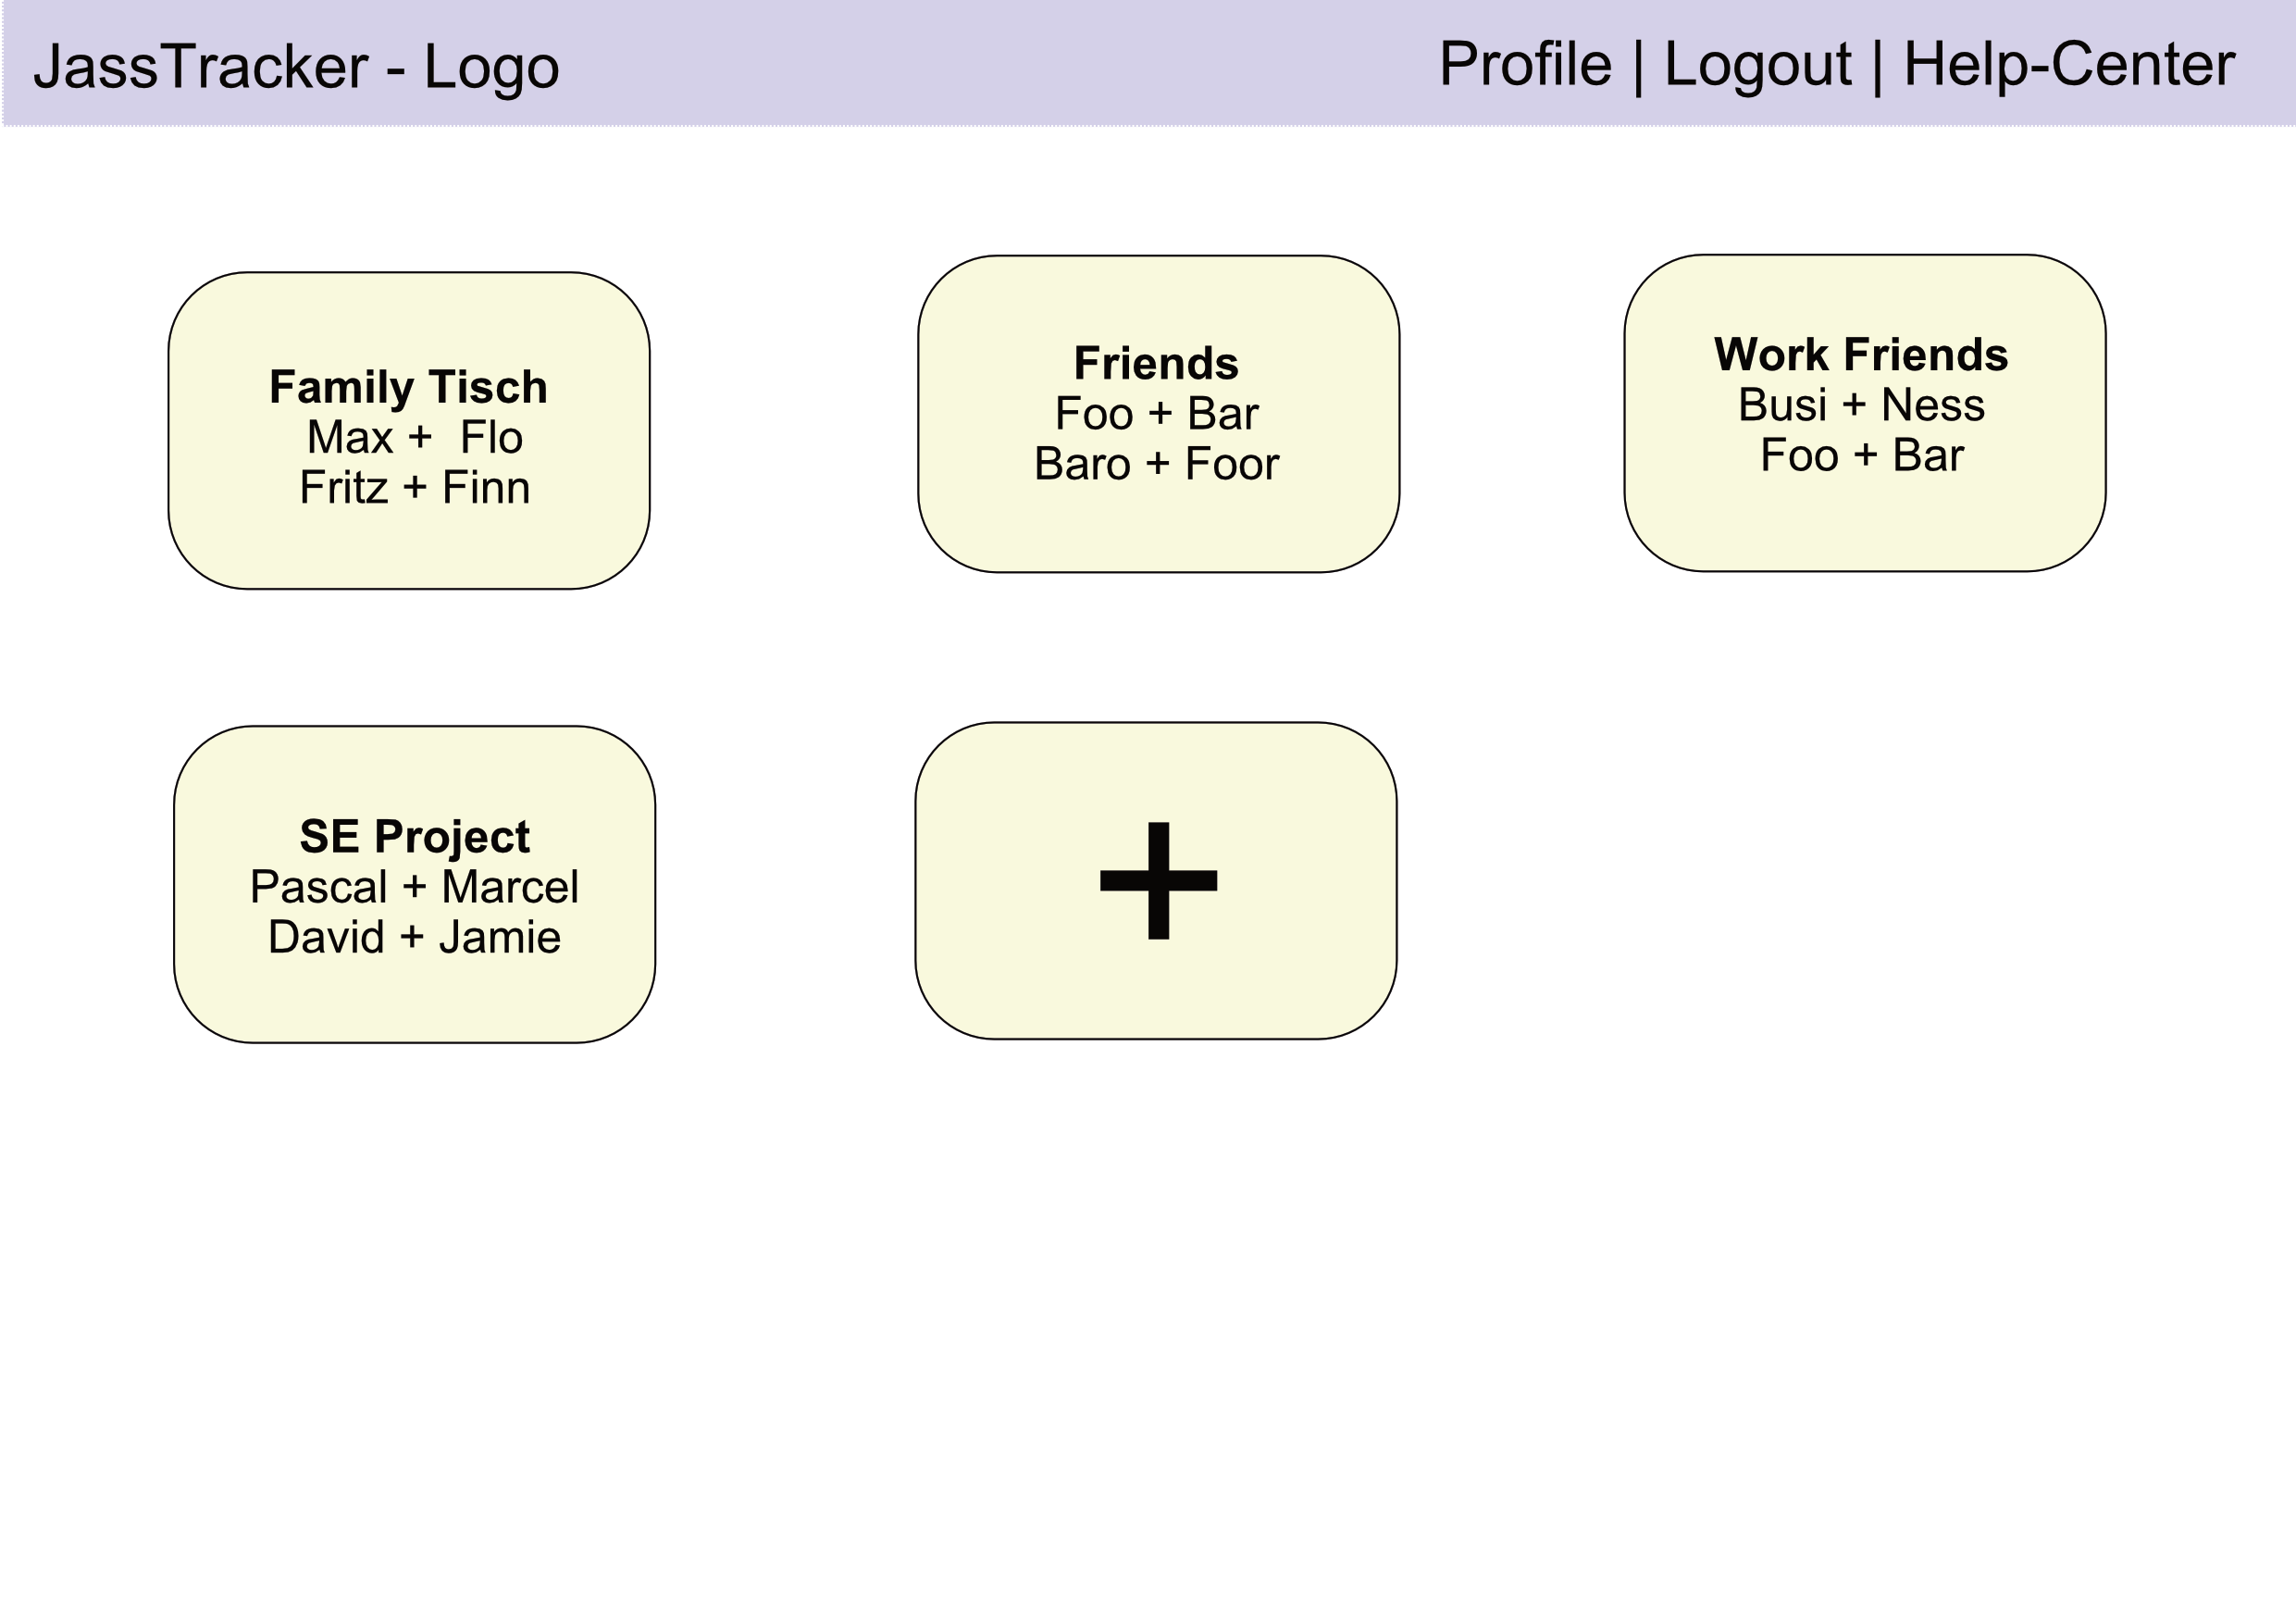
\includegraphics[height=10cm, width=\textwidth]{resources/mockups/mockup-table-overview}
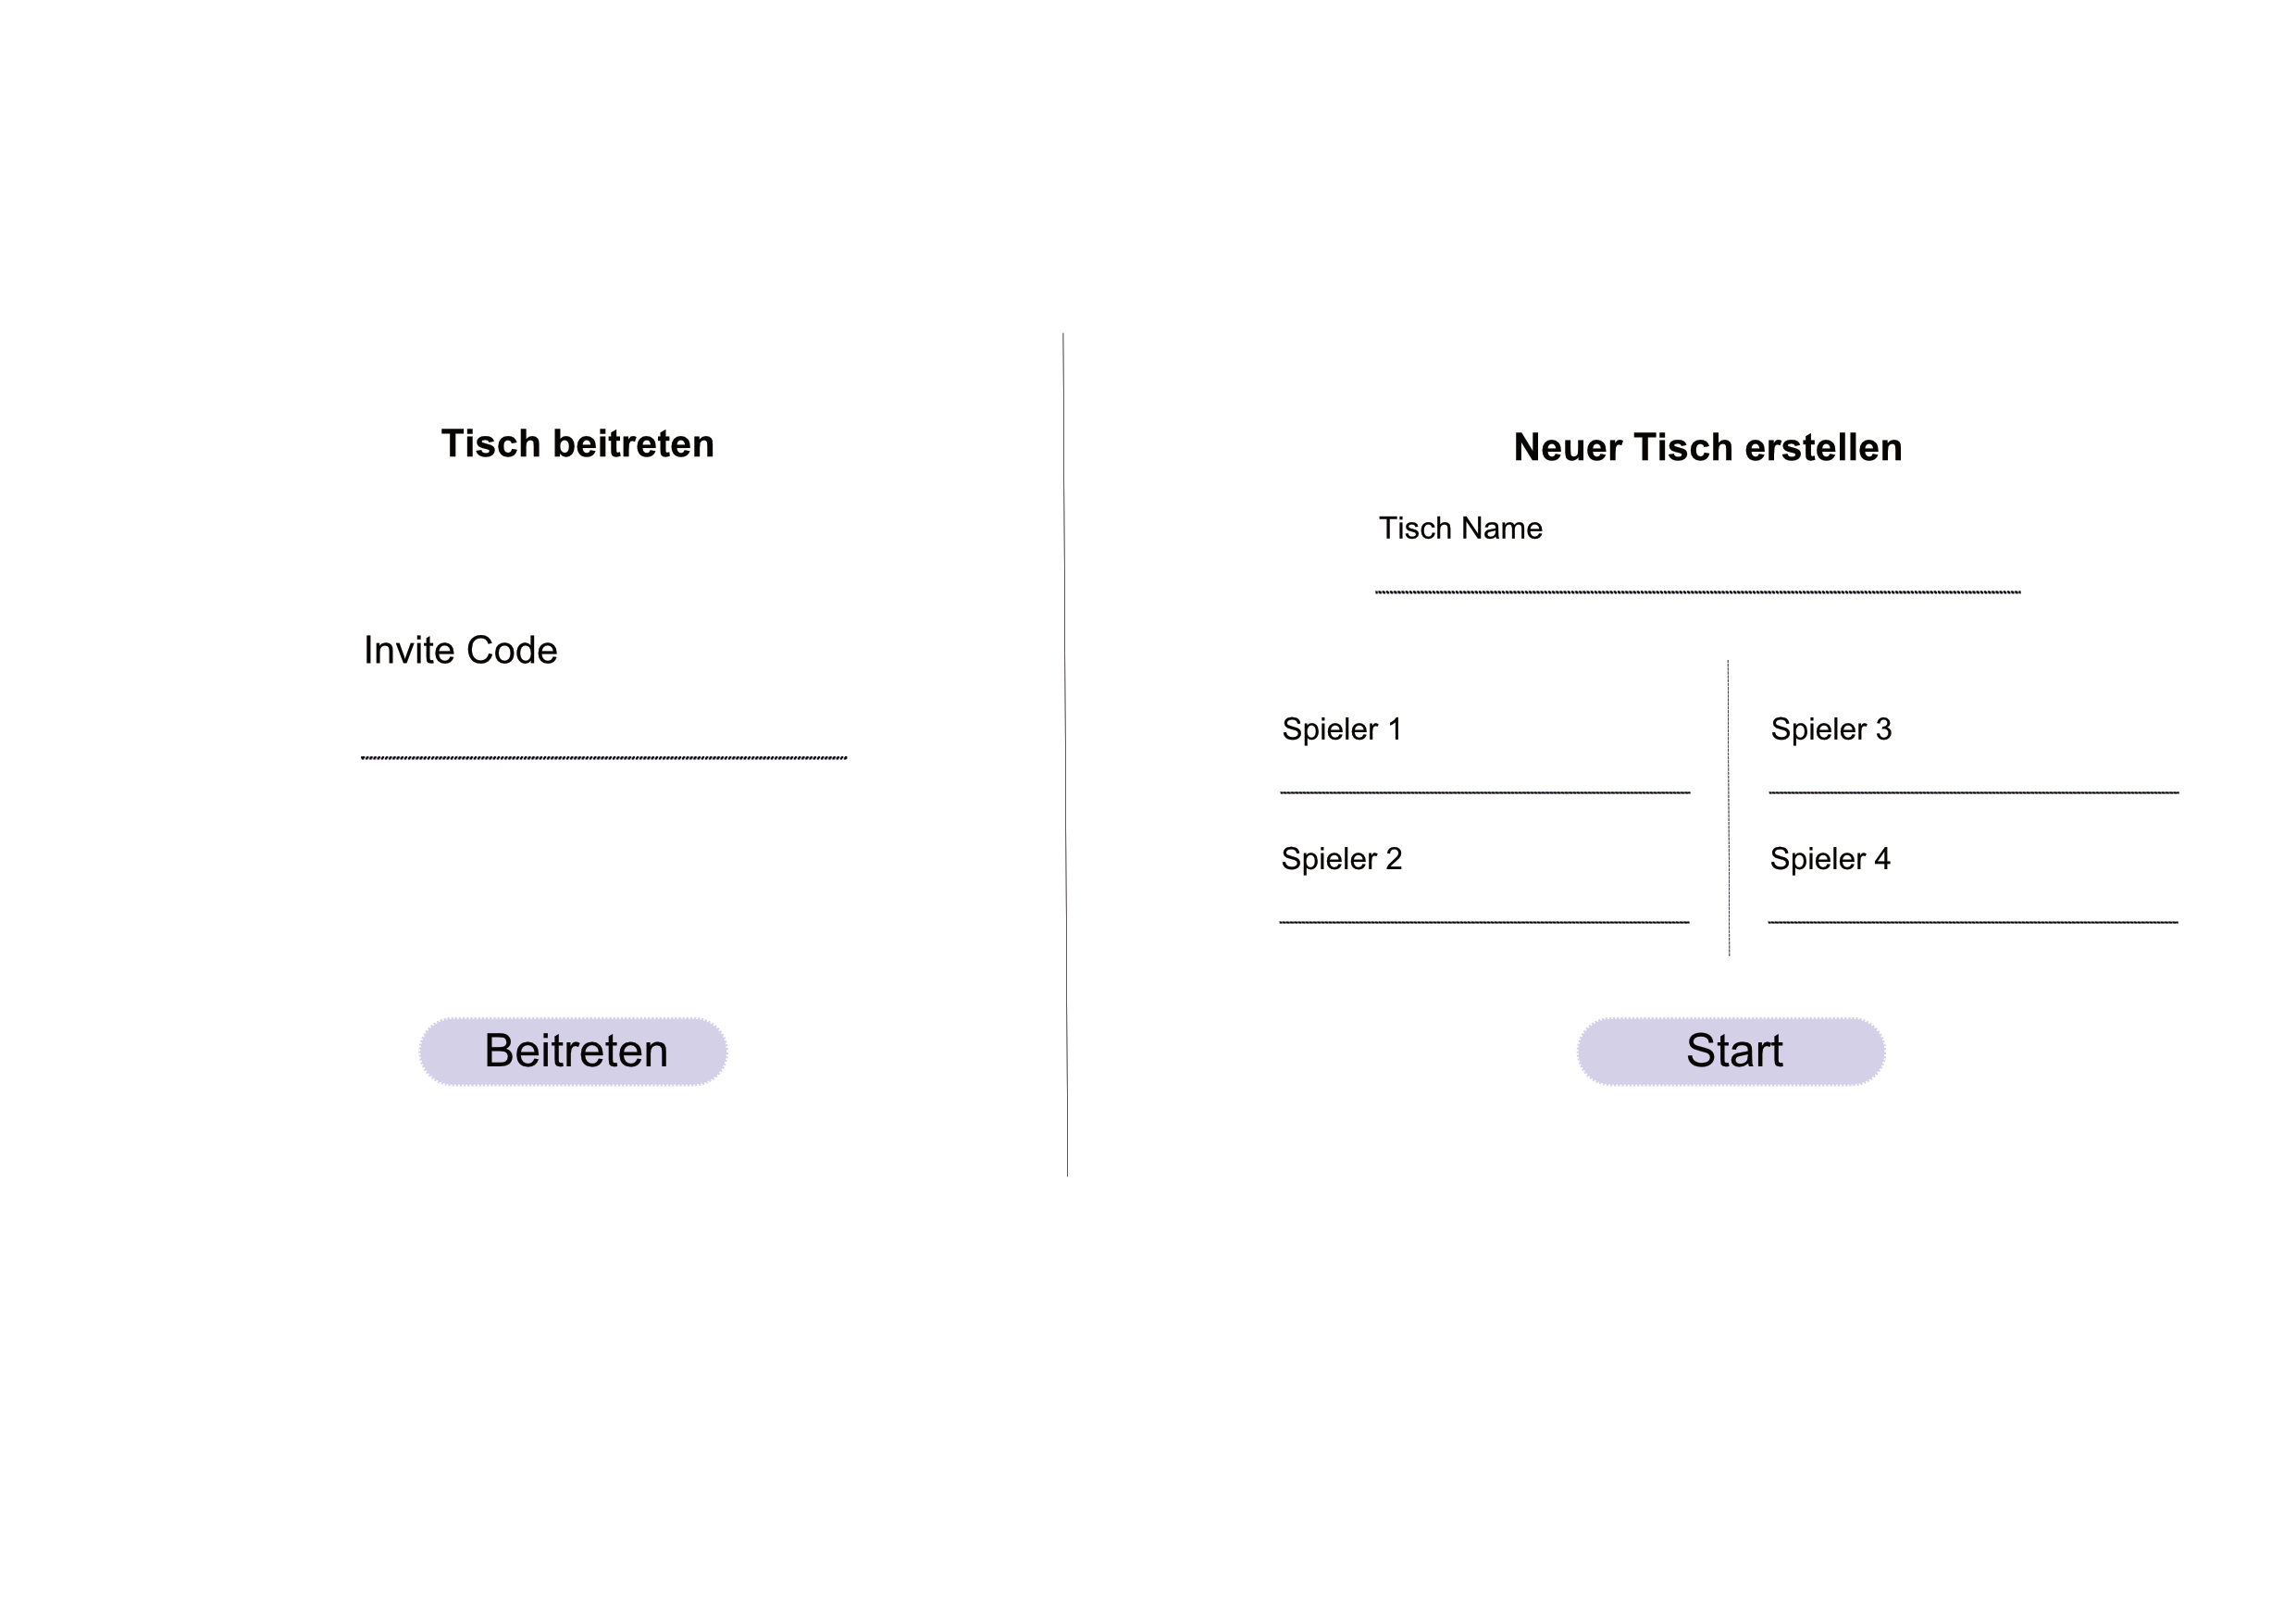
\includegraphics[height=10cm, width=\textwidth]{resources/mockups/mockup-create-new-table}
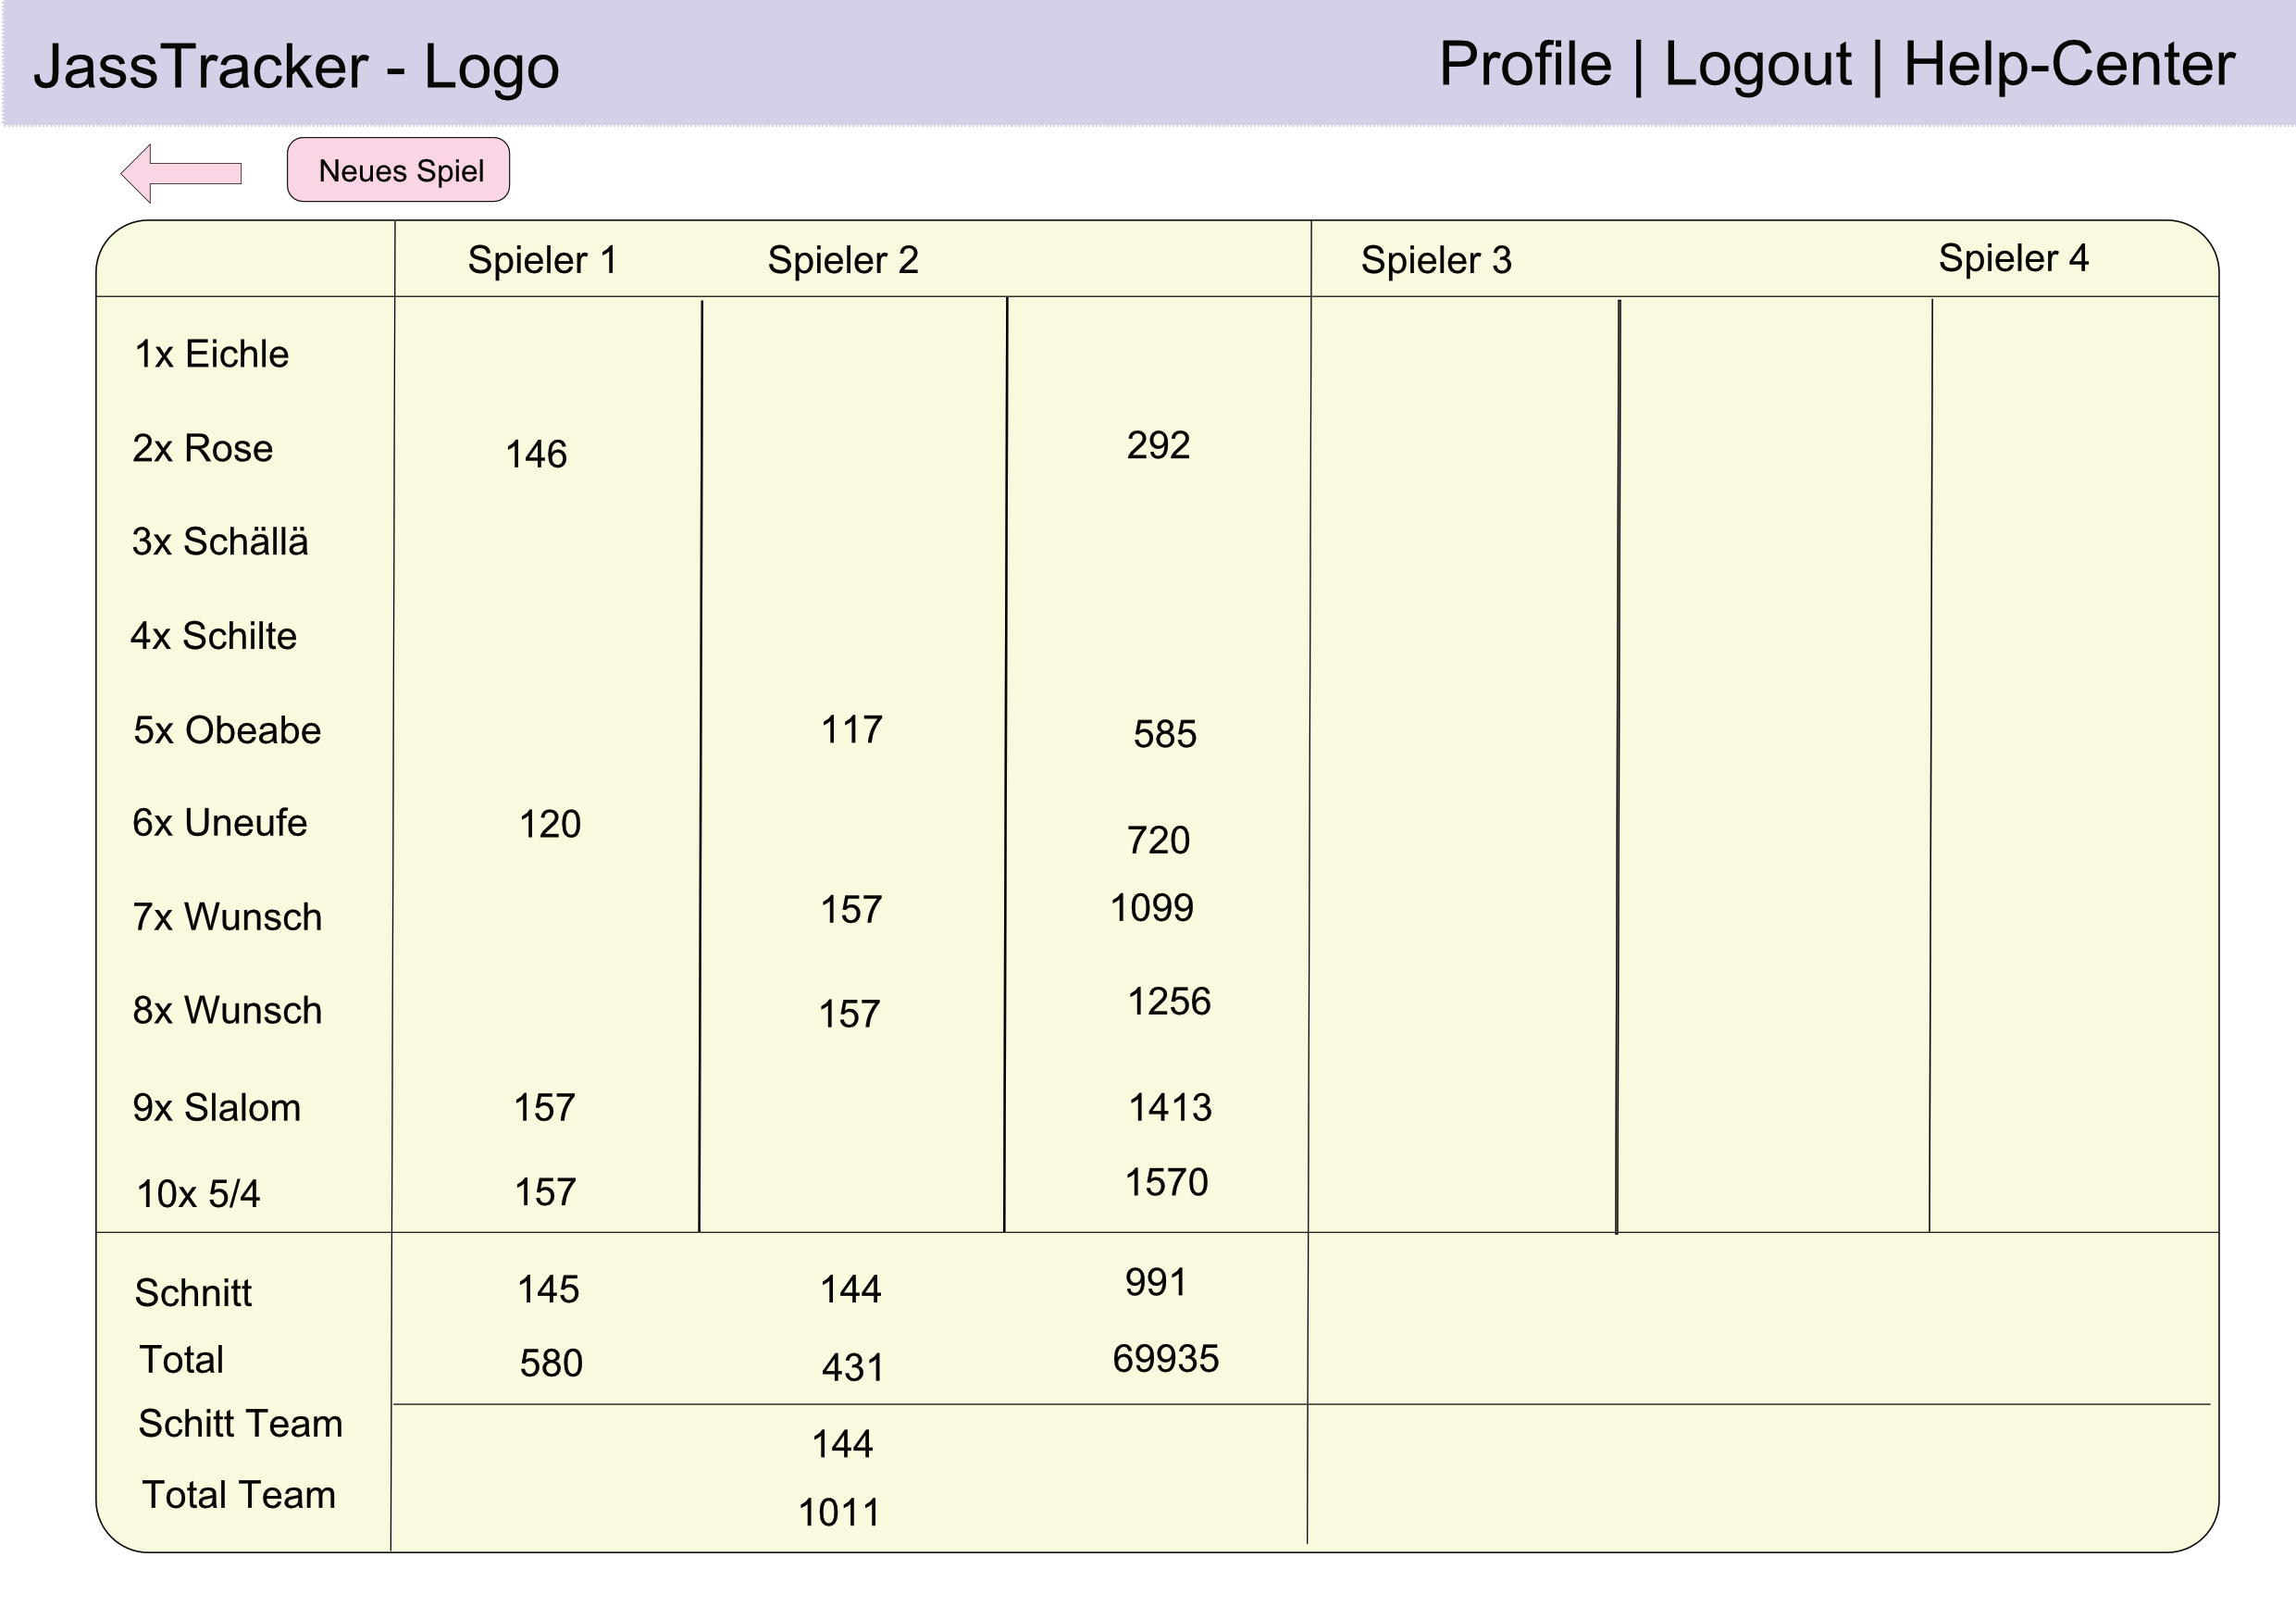
\includegraphics[height=10cm, width=\textwidth]{resources/mockups/mockup-scoreboard}
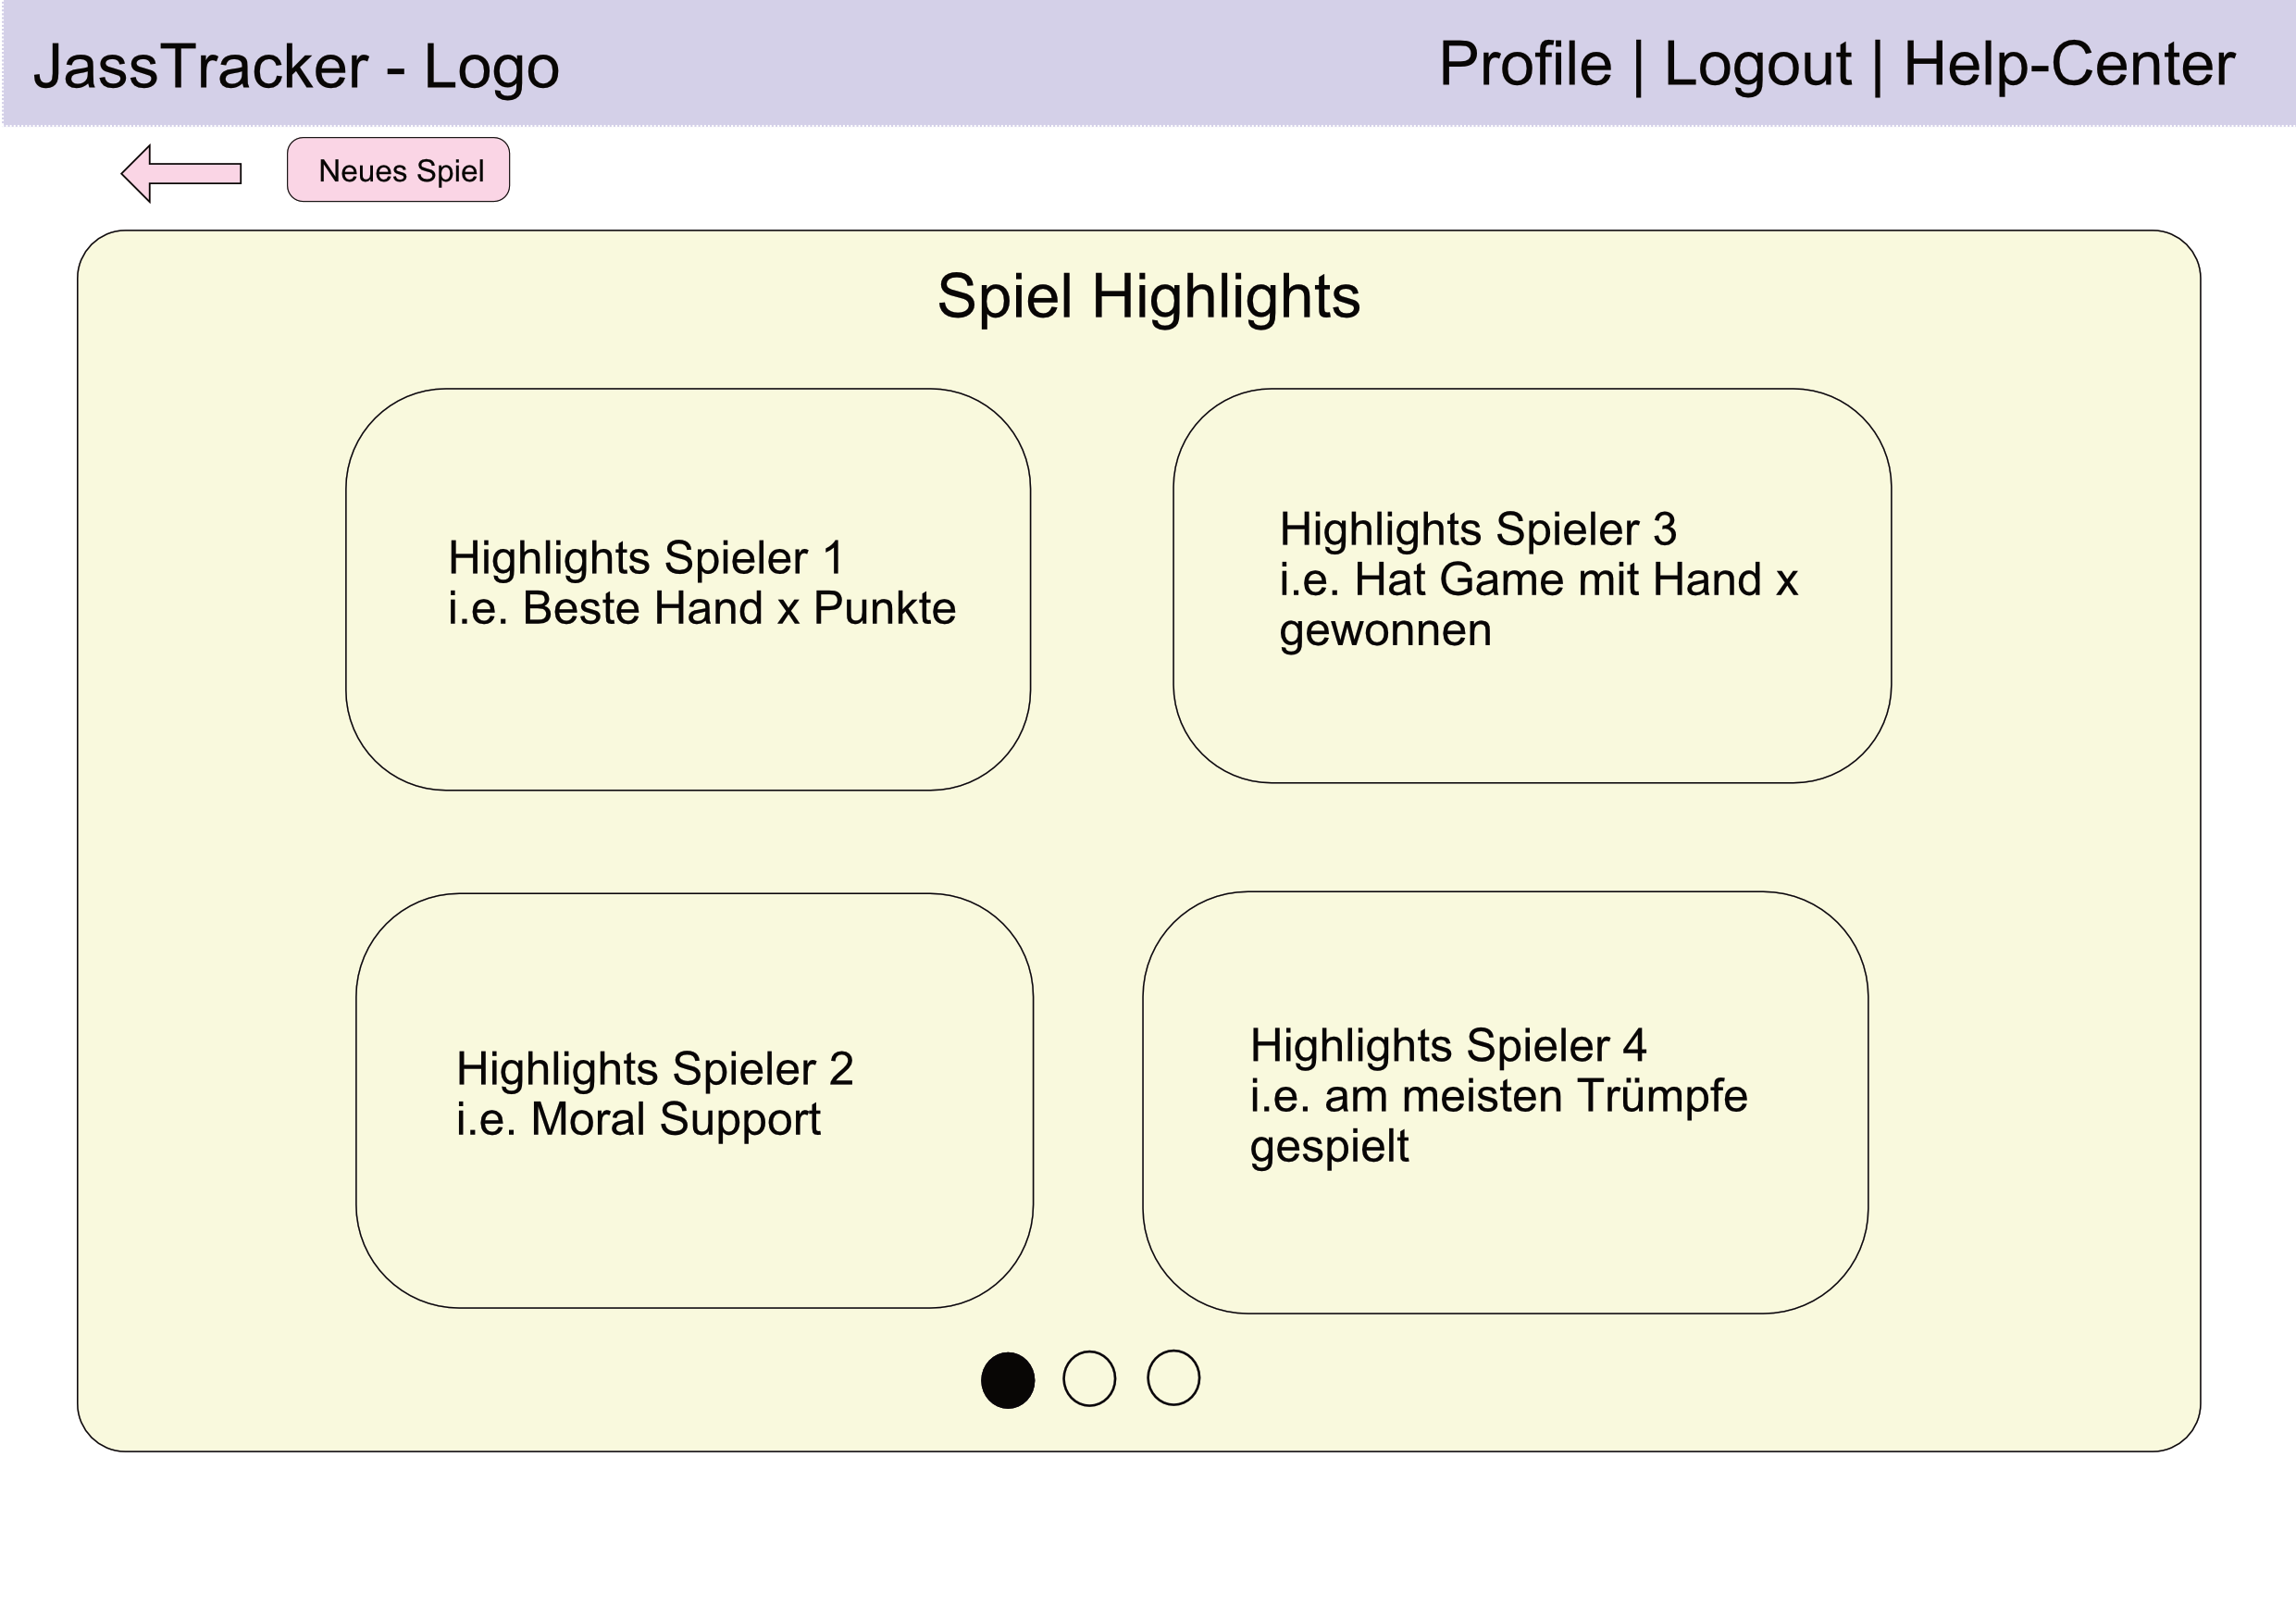
\includegraphics[height=10cm, width=\textwidth]{resources/mockups/mockup-eof-highlights}
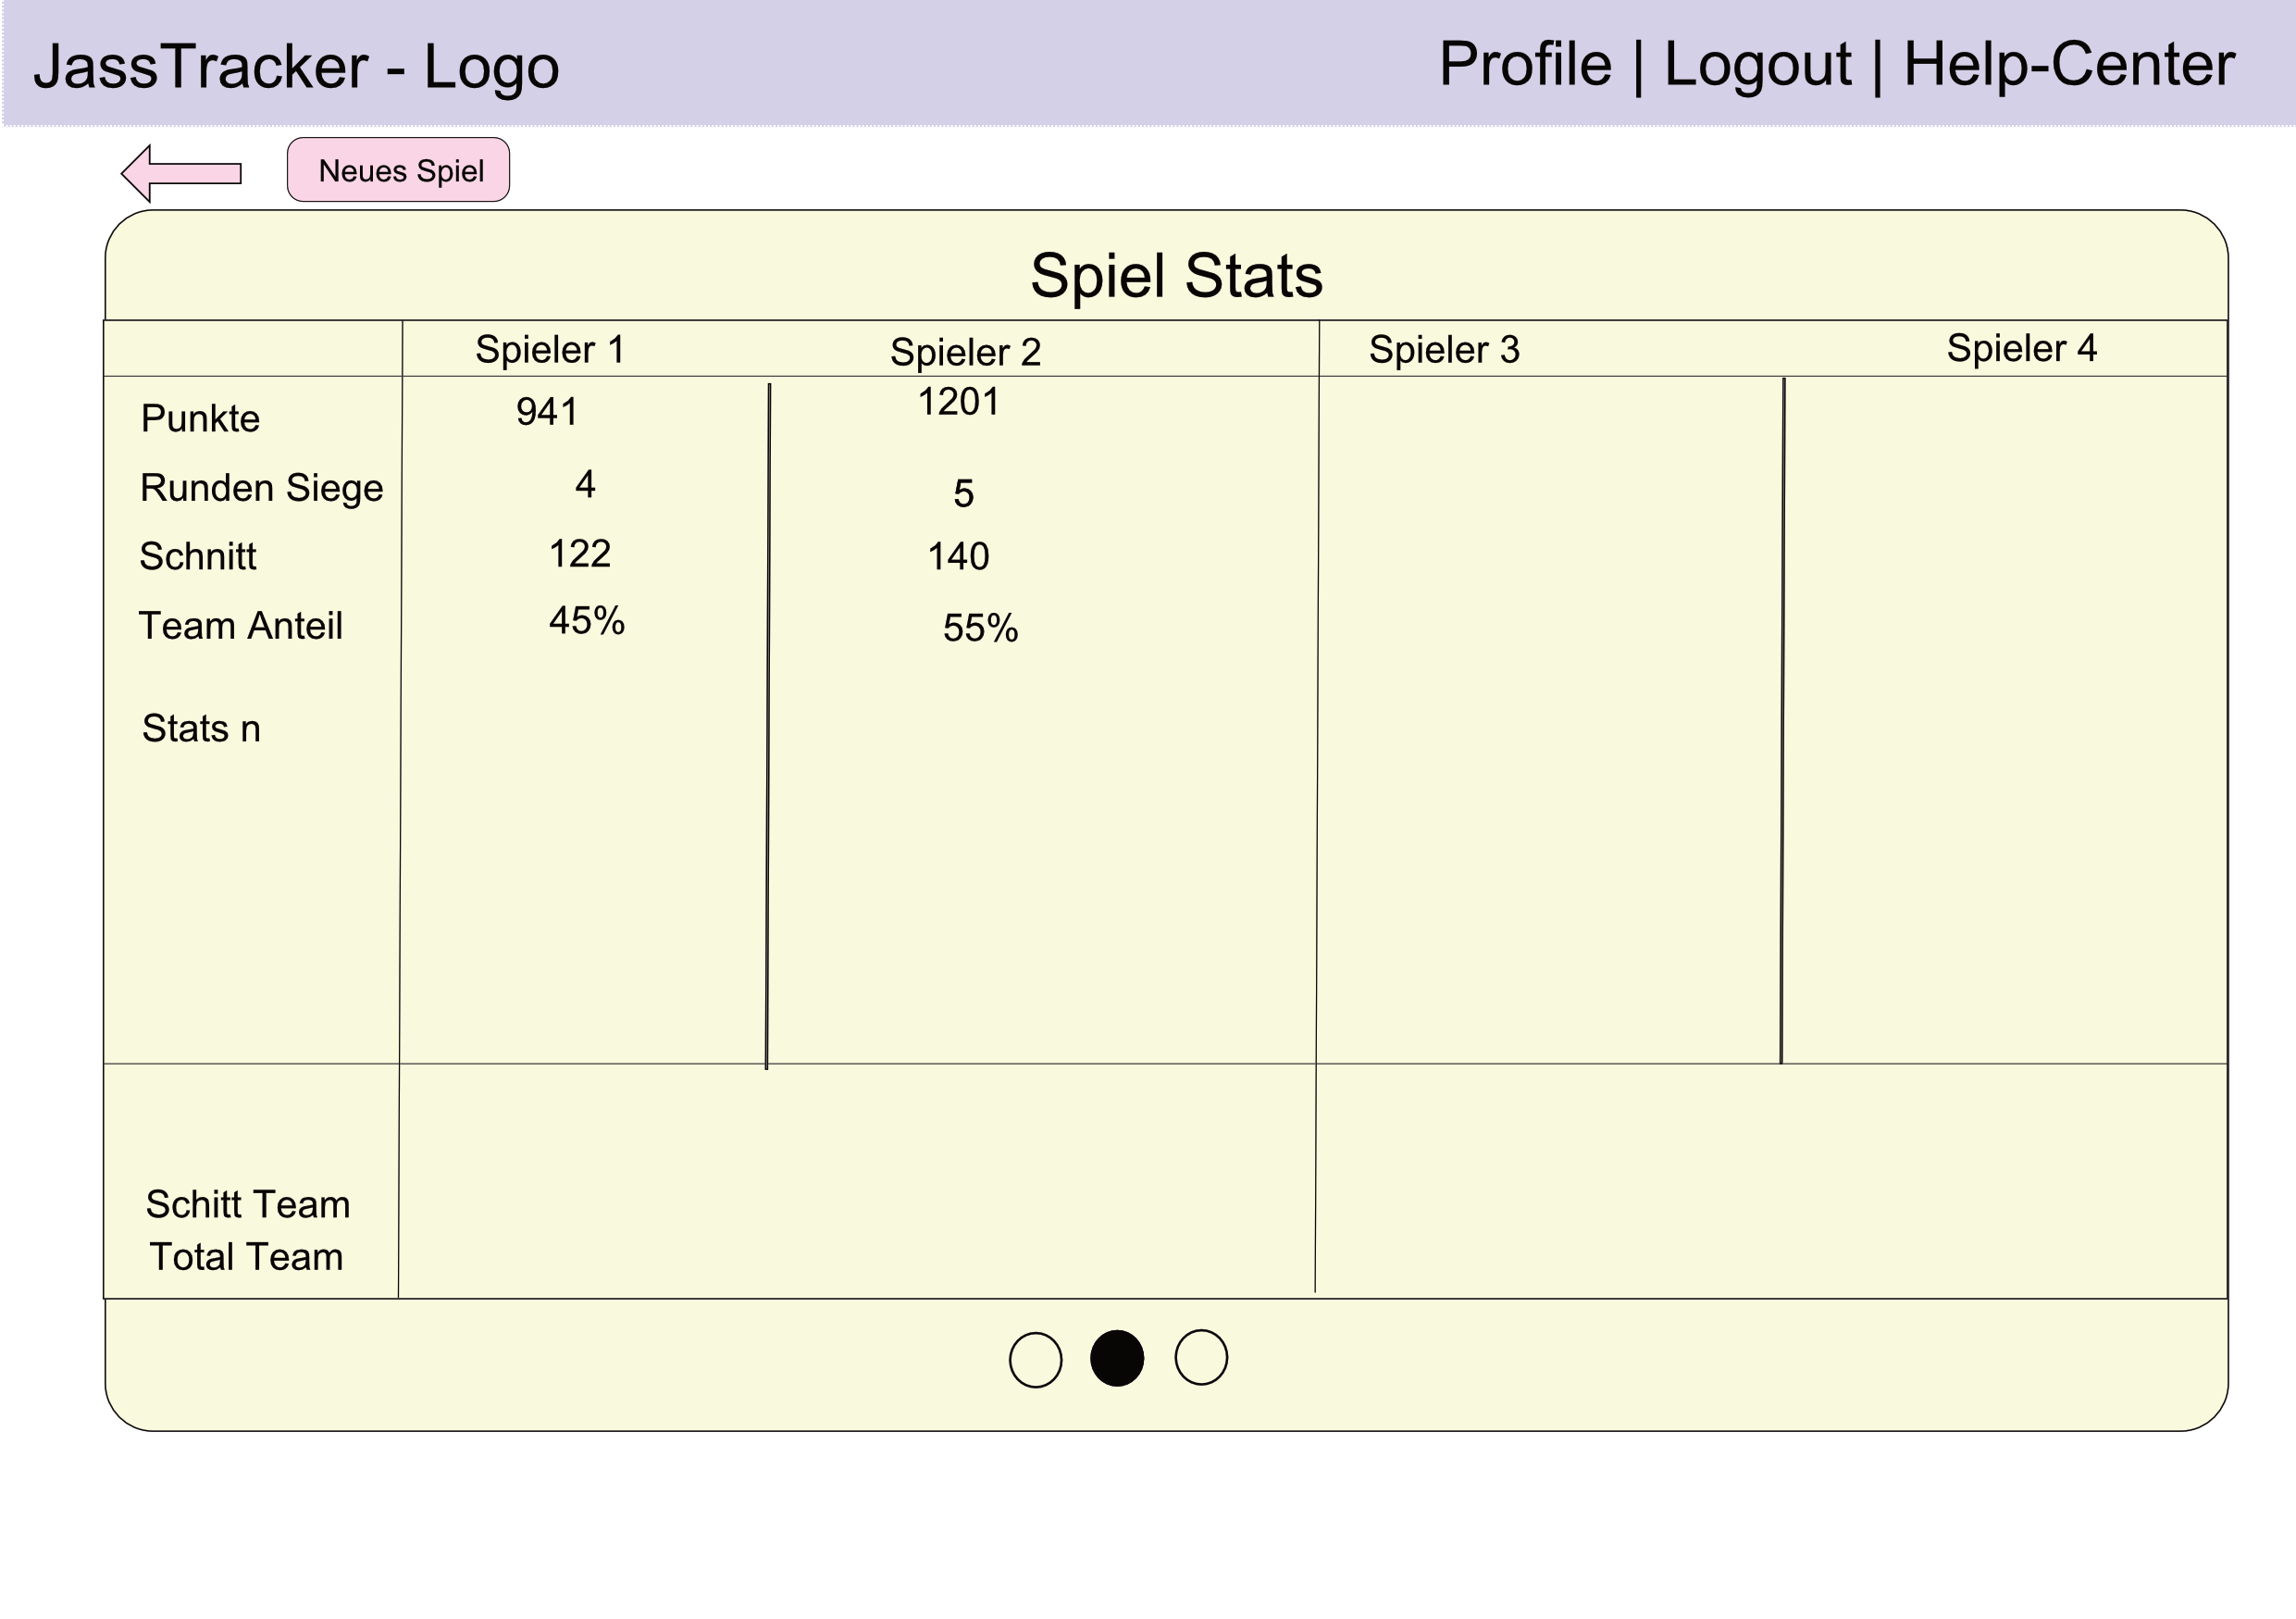
\includegraphics[height=10cm, width=\textwidth]{resources/mockups/mockup-eof-stats}
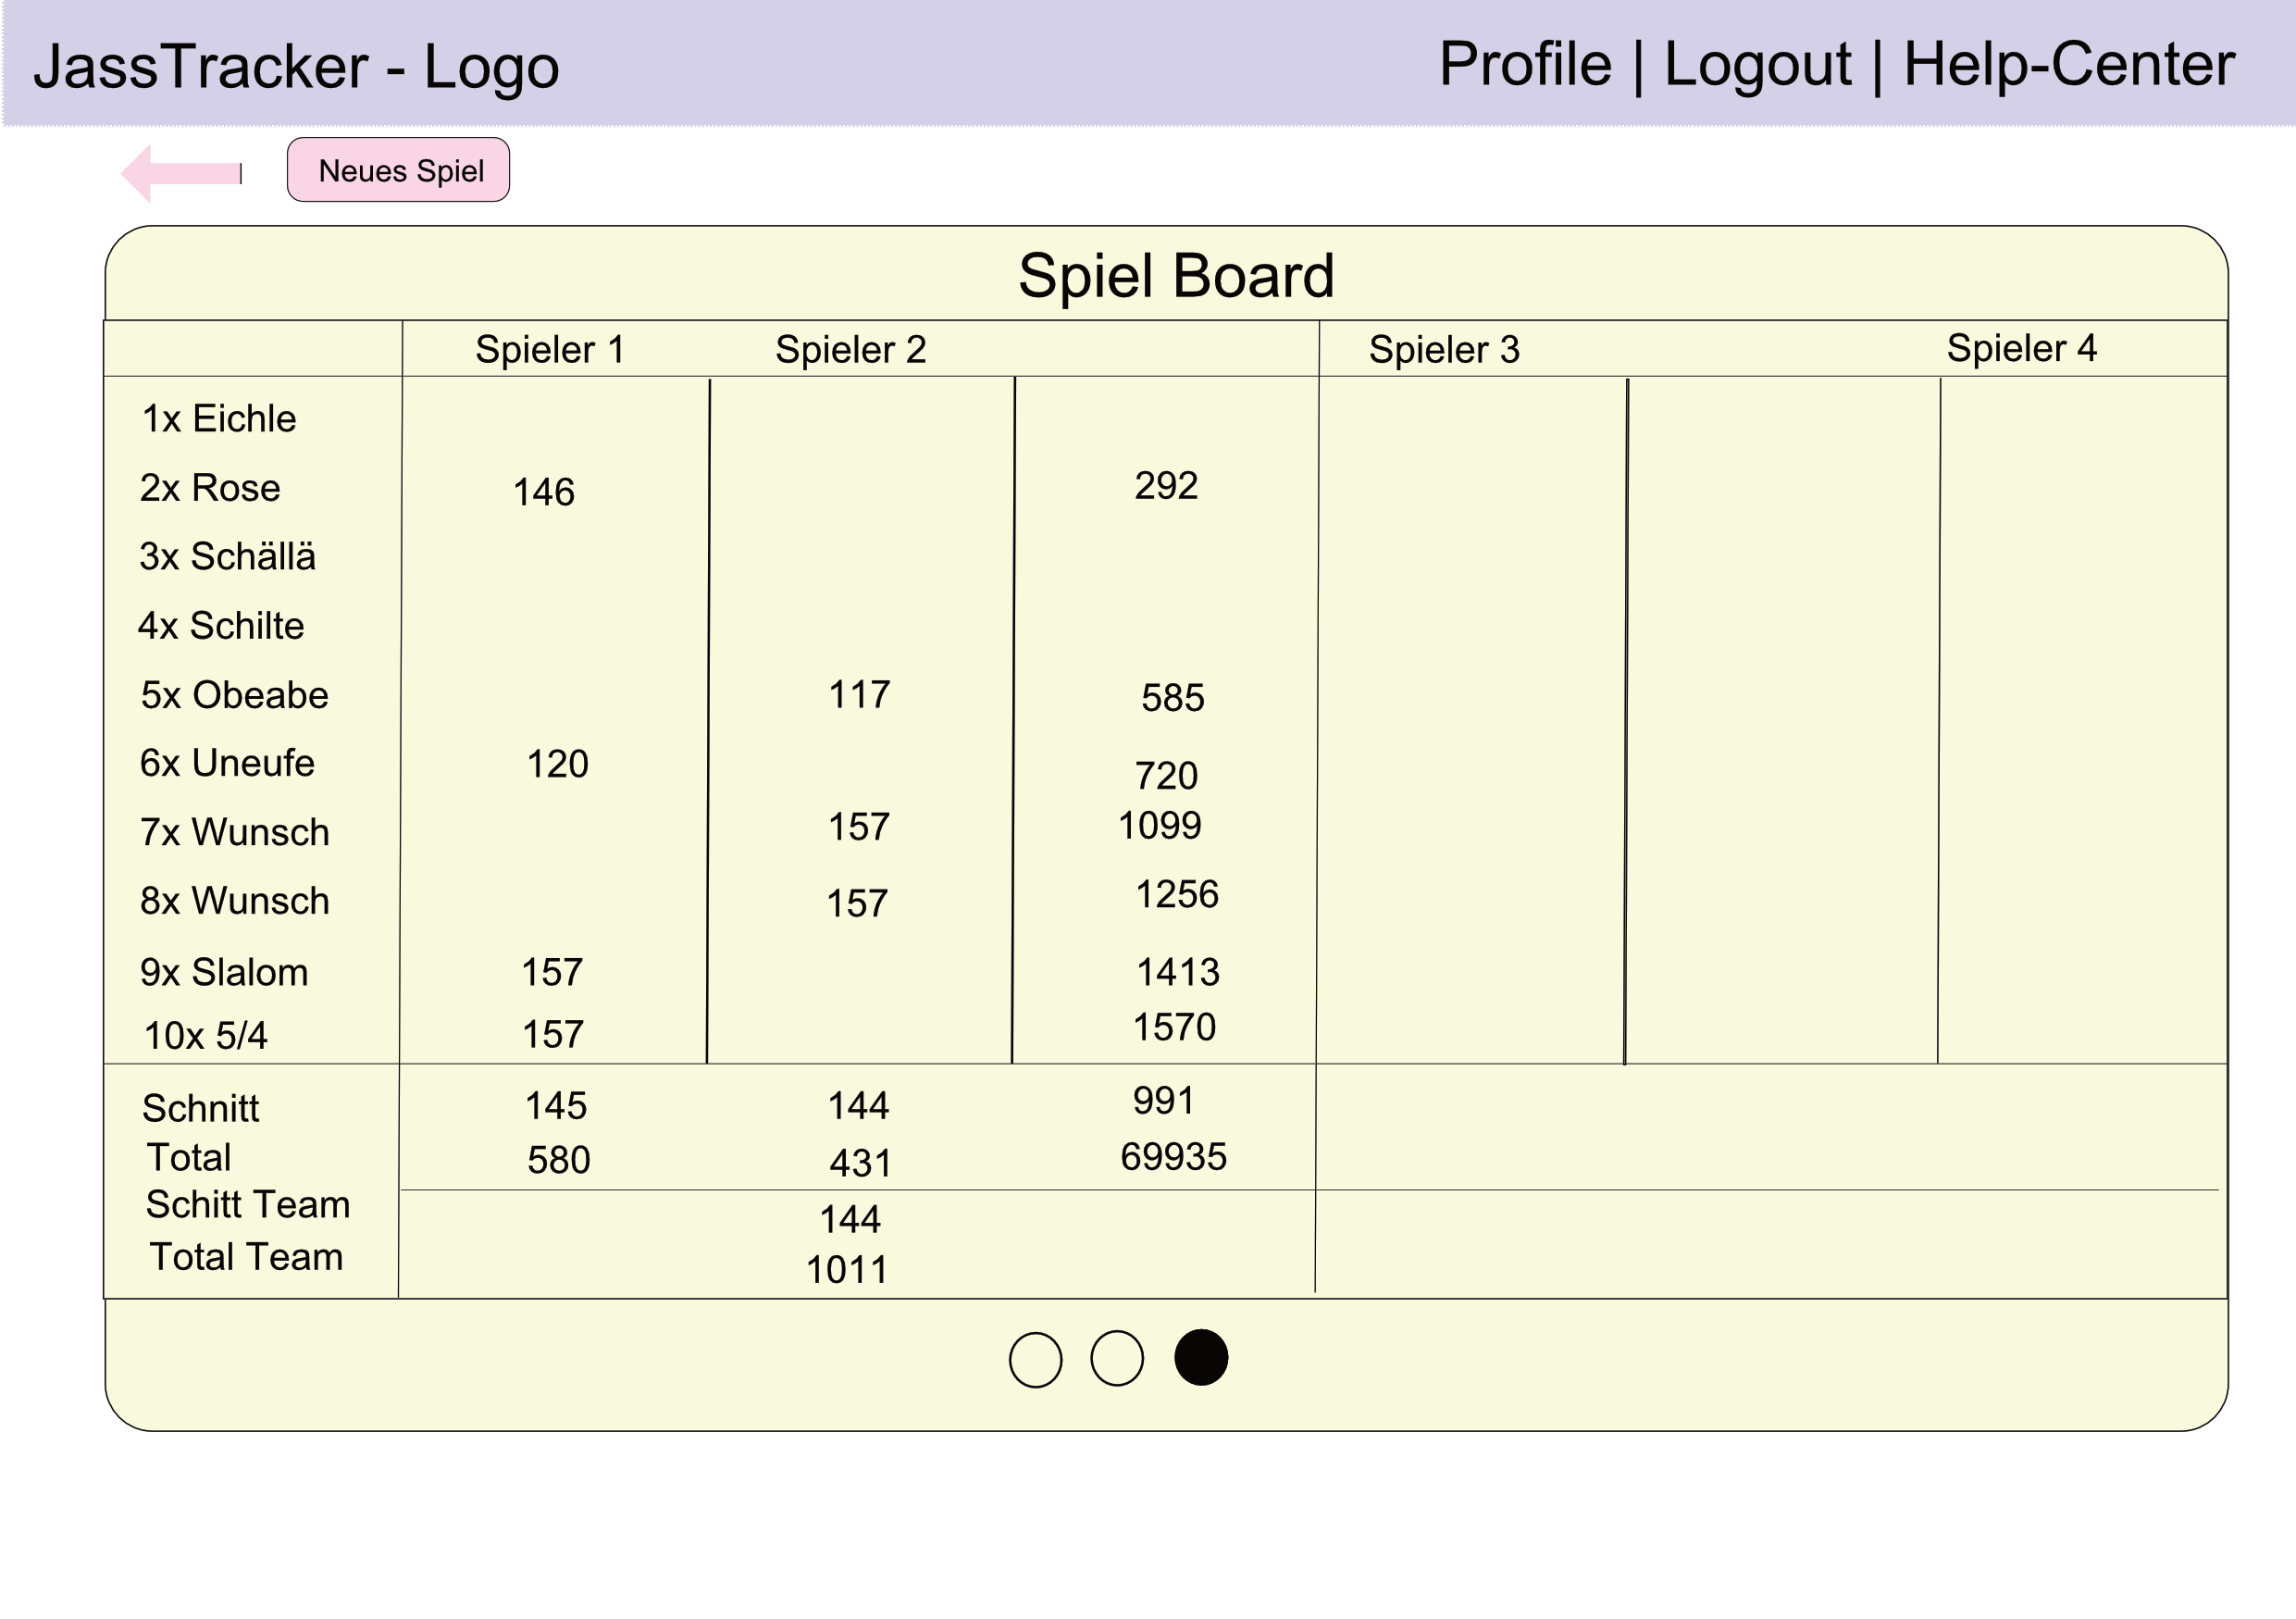
\includegraphics[height=10cm, width=\textwidth]{resources/mockups/mockup-eof-scoreboard}
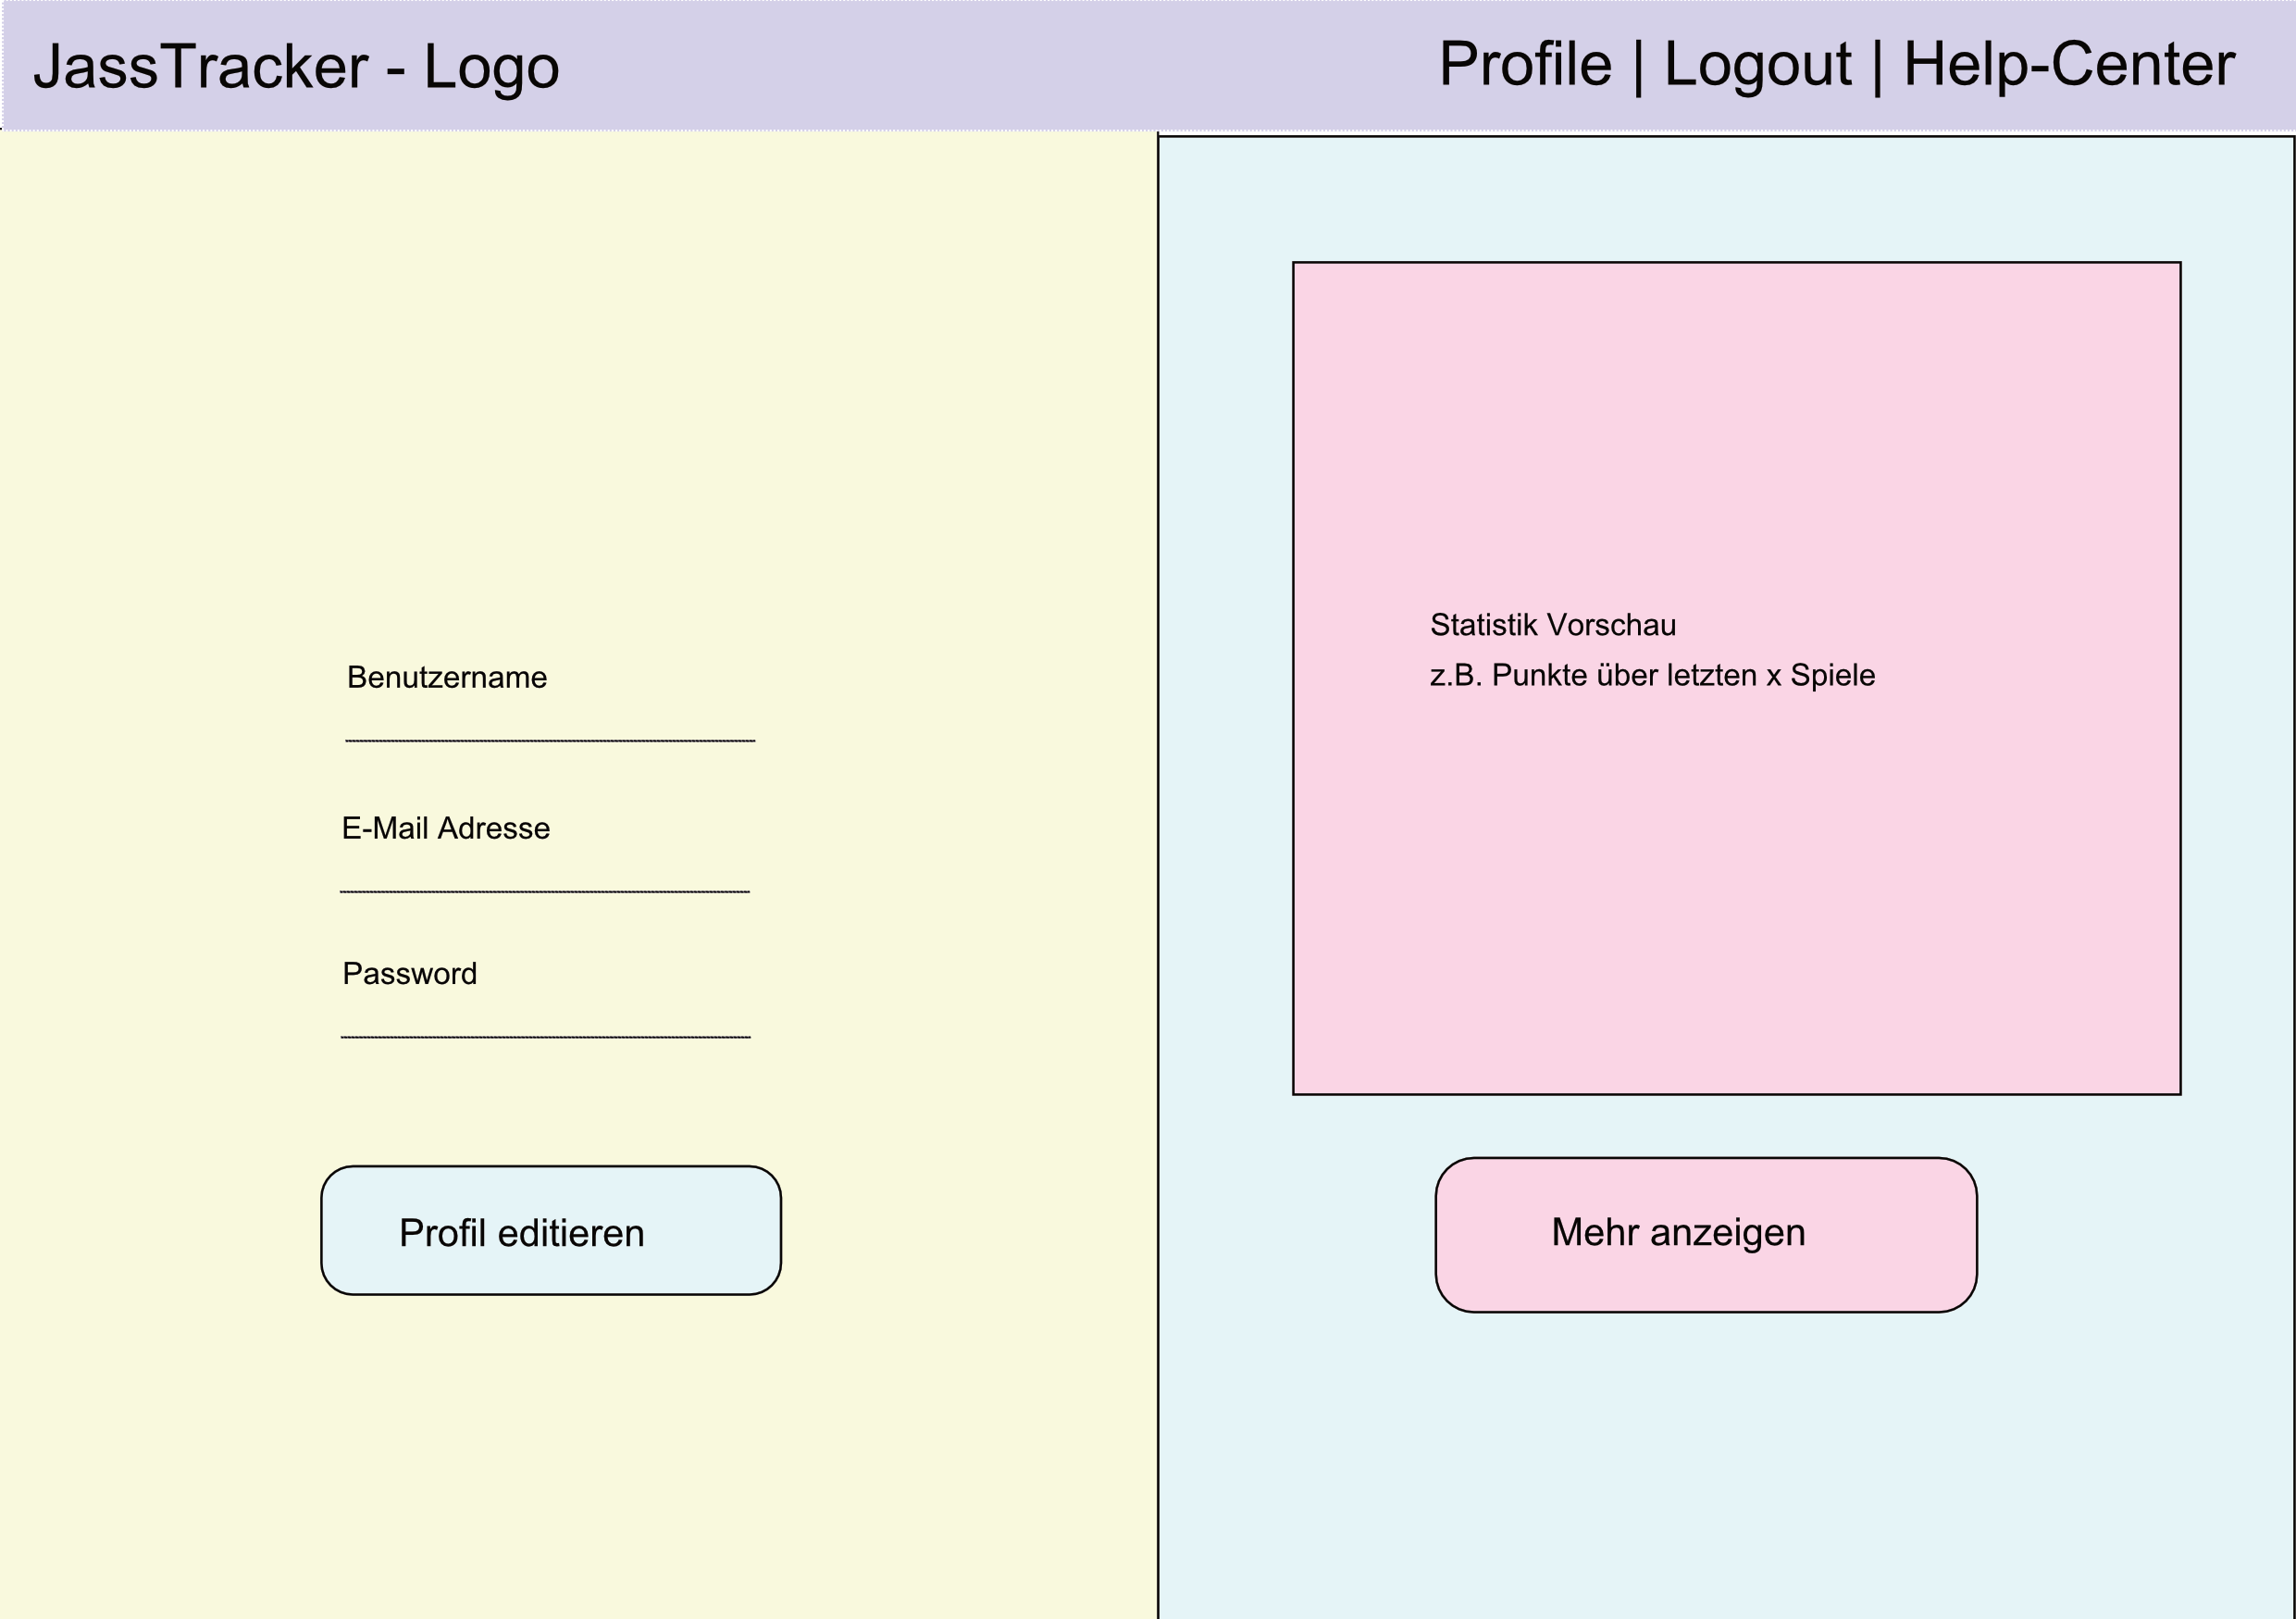
\includegraphics[height=10cm, width=\textwidth]{resources/mockups/mockup-profile-overview}
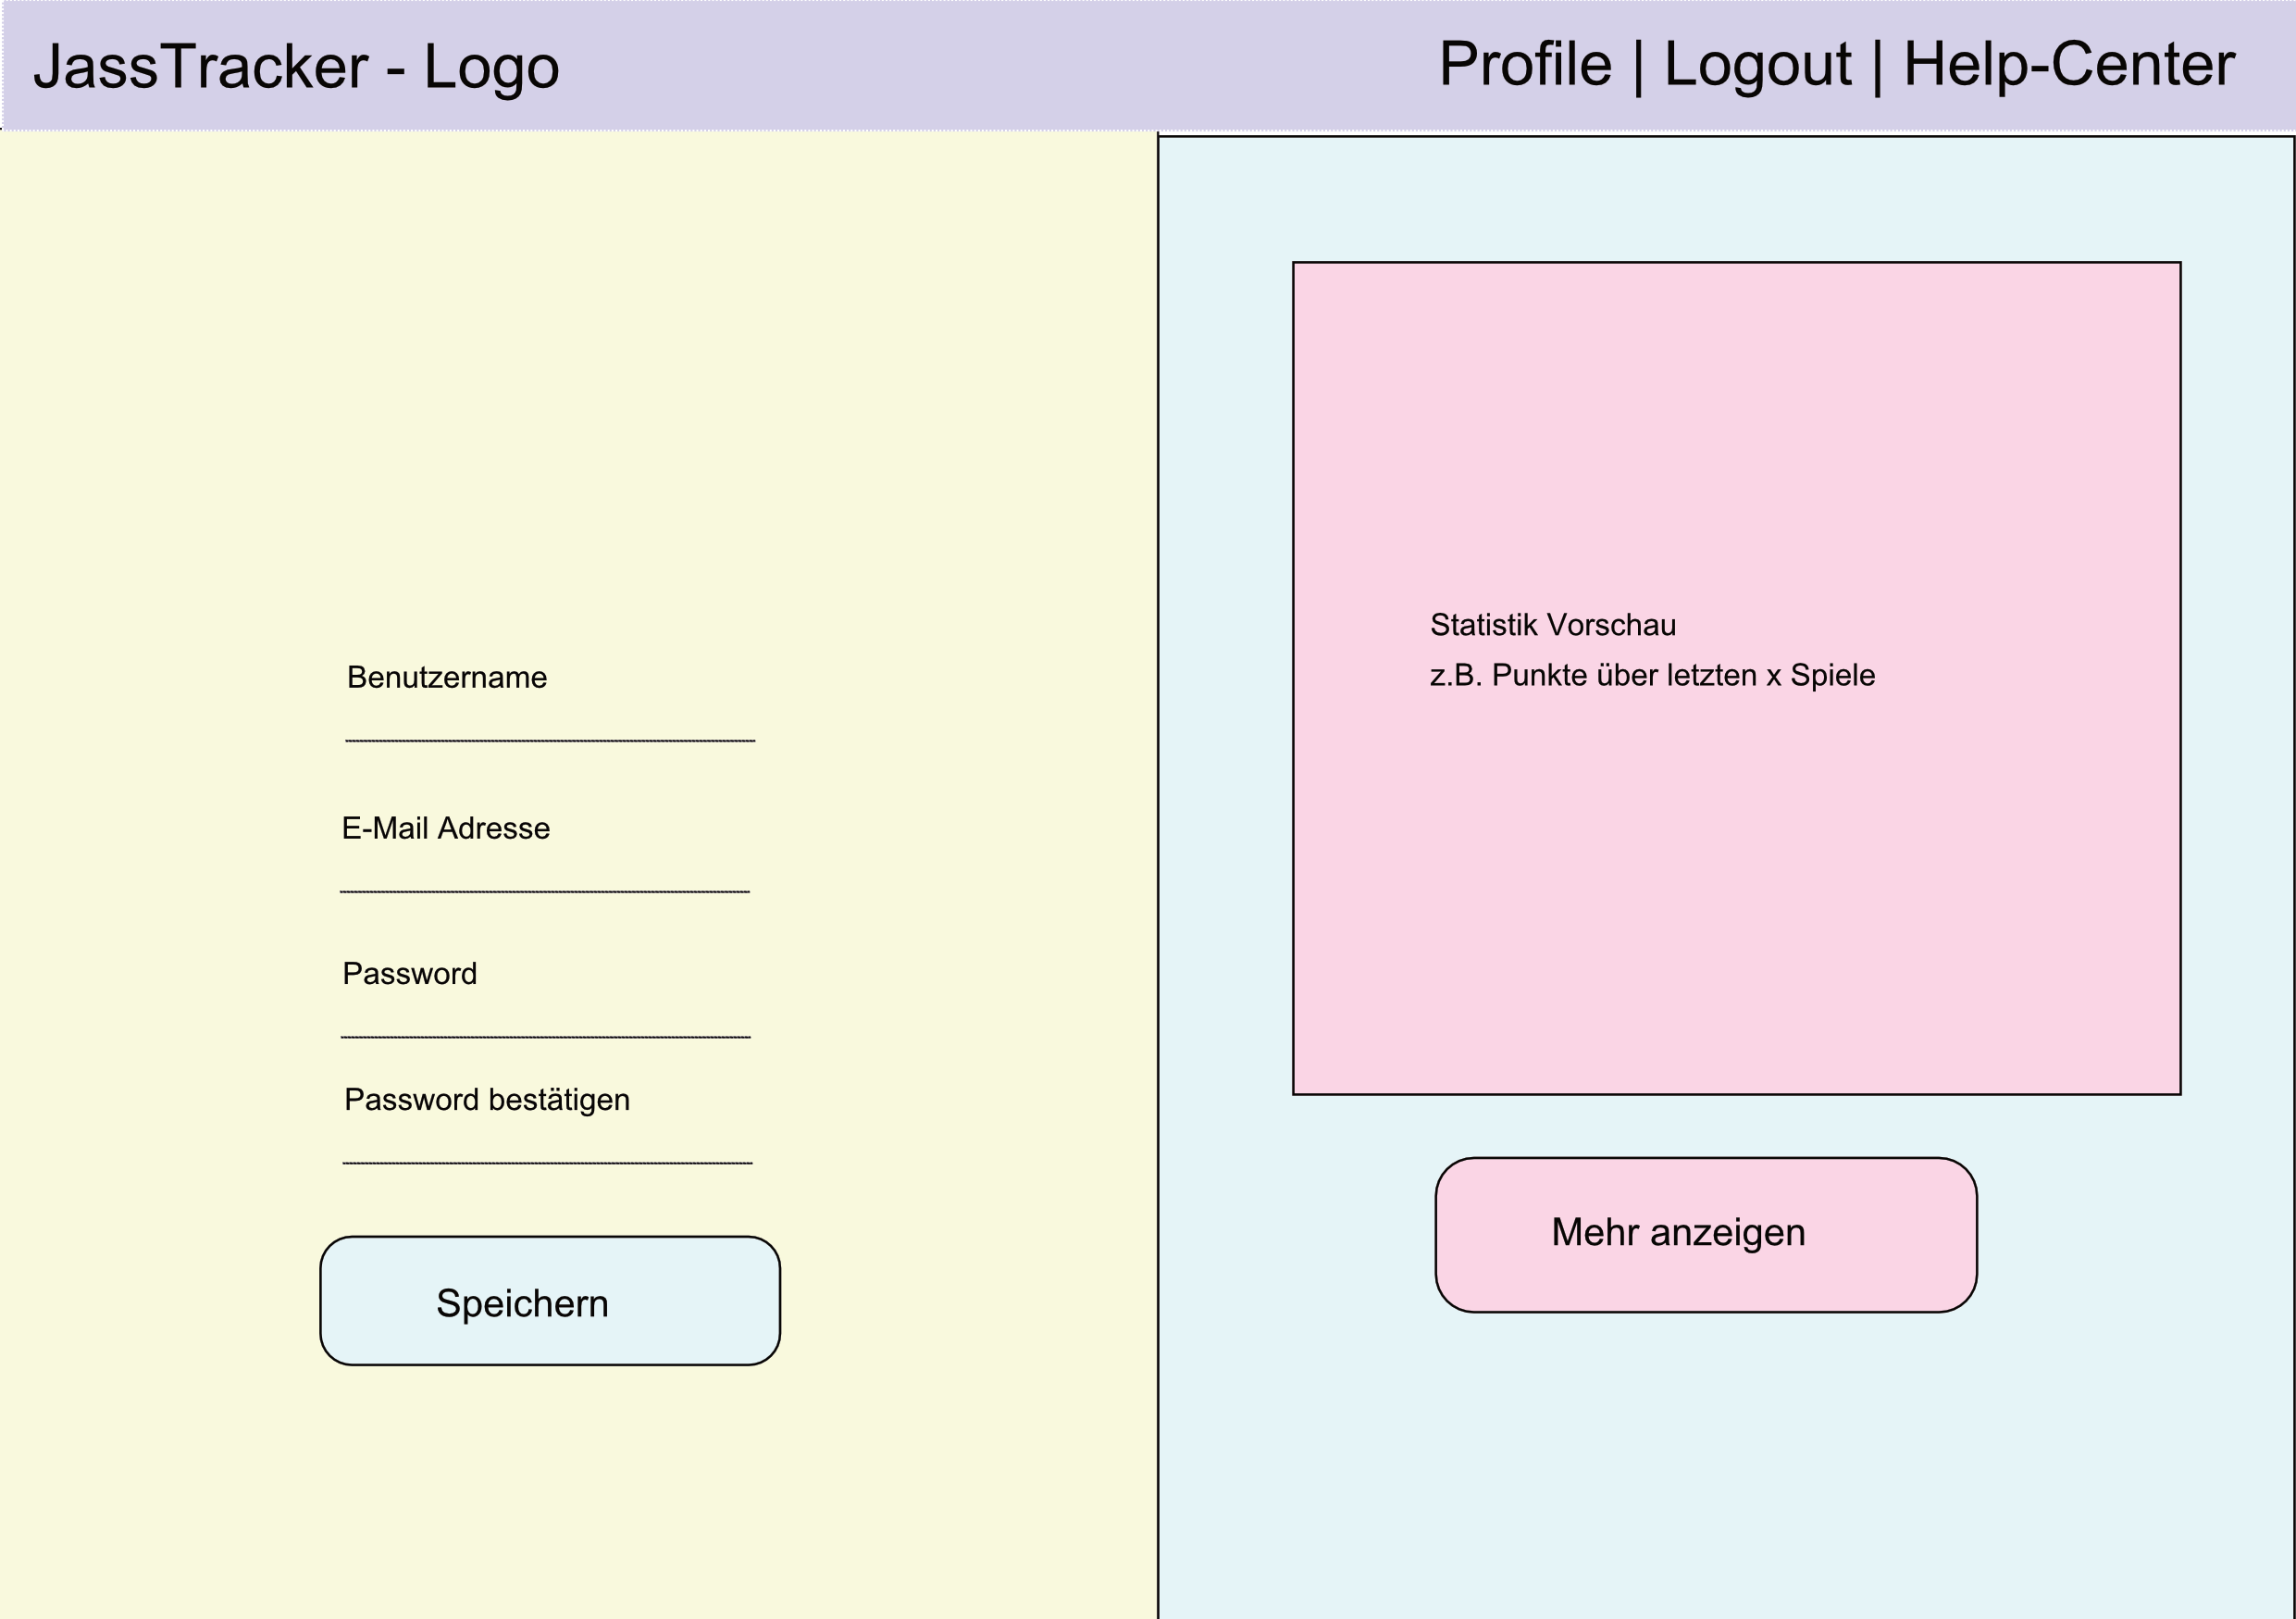
\includegraphics[height=10cm, width=\textwidth]{resources/mockups/mockup-profile-overview-edit}
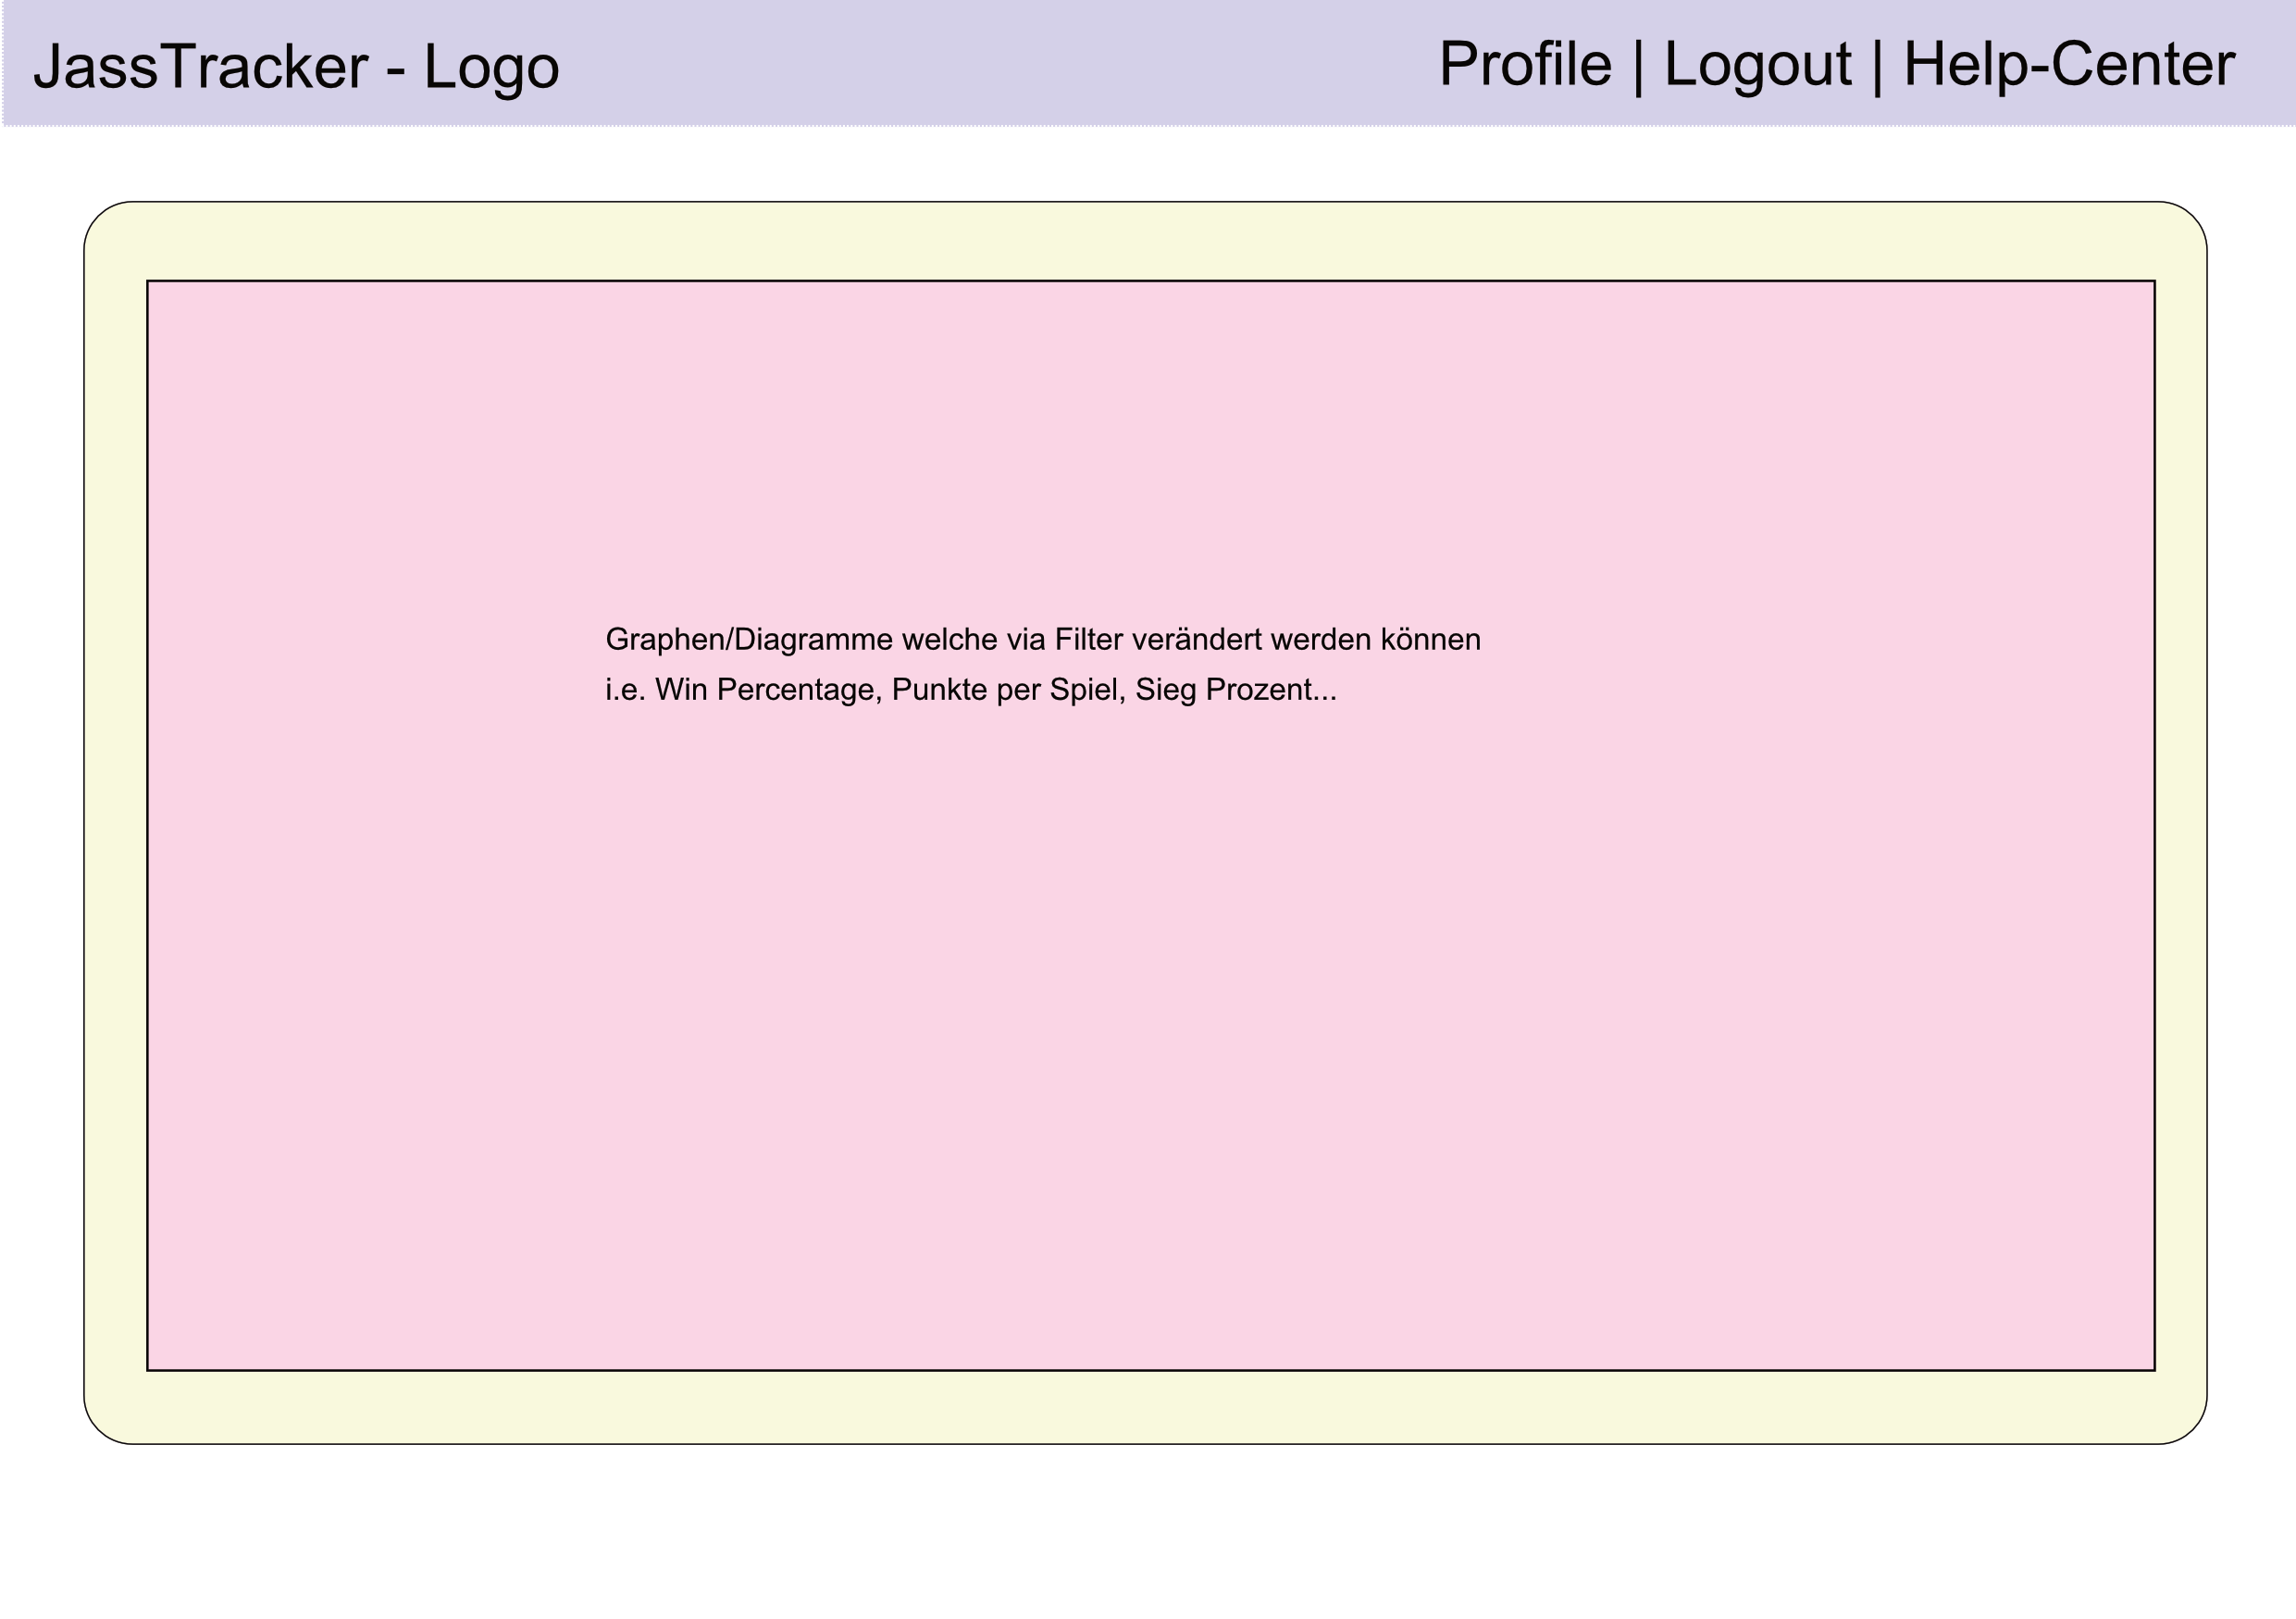
\includegraphics[height=10cm, width=\textwidth]{resources/mockups/mockup-player-stats}

\chapter{Domain Analysis}

\instructions{
    Describe the problem domain using a domain model as covered in the SEP1 module.
}
\chapter{Architecture}

\todo{KaTh}
\chapter{Quality Measures}

\section{Working with Git}
\begin{itemize}
    \item We use conventional commits
    \item We use Merge Requests in GitLab, direct pushes to master are forbidden
    \item We rebase our commits locally and create a merge commit when merging into master
\end{itemize}

\section{Definition of Done (DoD)}

\subsection{Feature (Defect / Story)}
\begin{itemize}
    \item Acceptance criteria / issue of user story is met
    \item Code follows best practices and guidelines
    \item No TODOs without a issue number are allowed
    \item Project builds without errors or warnings
    \item Tests are written and all tests are passing
    \item Peer Code Review performed
    \item Project deployed on the test environment identical to production platform
    \item Documentation updated
    \item Associated with epic and release
    \item Hours worked on are logged correctly
\end{itemize}

\subsection{Sprint}
\begin{itemize}
    \item DoD of each item included in the sprint is met
    \item Product backlog updated
    \item Sprint has a defined goal
    \item Sprint marked as ready for the production deployment by the Product Owner
\end{itemize}

\subsection{Release}
\begin{itemize}
    \item Release is documented and all continuing tasks are associated
    \item Code complete
    \item Environments are prepared for release
    \item QA is done \& all issues resolved
    \item Manual tests pass
    \item Check that no unfinished work has been left in any development or staging environment.
\end{itemize}

\section{Definition of Ready (DoR)}

\subsection{Defect}
\begin{itemize}
    \item Steps to reproduce
    \item Severity
    \item Screenshots
\end{itemize}

\subsection{Story}
\begin{itemize}
    \item Use-Case (e.g.\ view current score)
    \item Estimate
    \item Epic link
    \item Acceptance criteria list specified
    \item Should be doable within a week, otherwise try to split it
\end{itemize}

\section{Test Concept}
\subsection{Unit Tests}
\begin{itemize}
    \item Business Logic will be unit tested
    \item Runs on every push to GitLab, merging is blocked until failing tests are fixed
    \item Automated
\end{itemize}

\subsection{Integration Tests}
\begin{itemize}
    \item Framework / technology dependent code will be integration tested
    \item Runs on every push to GitLab, merging is blocked until failing tests are fixed
    \item The web API layer is tested by using \href{https://ktor.io/docs/testing.html}{Ktor testing}, allowing us to verify our REST endpoints
    \item The data access layer is tested by using \href{https://www.testcontainers.org/}{Testcontainers}, allowing us to use a real PostgreSQL DB in our tests
    \item Automated
\end{itemize}

\subsection{Usability Tests (See Chapter~\ref{ch:uxtesting})}
\begin{itemize}
    \item Project will be given to multiple people for testing (hallway testing)
    \item Testers should be able to use website without having to ask any questions
    \item Manual
\end{itemize}

\subsection{System Tests}
\begin{itemize}
    \item How full System works together - how components interact
    \item Influenced by usability testing
    \item Manual
    \item \href{https://www.cypress.io}{Cypress} was evaluated for automated end-to-end testing, but we came to the conclusion that our time is better invested in manual usability testing and actually improving our app.
\end{itemize}

\section{Continuous Integration and Deployment}
We use GitLab for continuous integration and have a pipeline which runs on every commit and builds both frontend and backend.
For the backend, tests are run and a linter for the frontend.
If all jobs succeed, a Docker image is built, pushed to the registry and tagged with the current branch name.
Once a merge request is merged into the master branch the pipeline is run again and a Docker image tagged with latest is built.
If that succeeds the new image is automatically deployed to our staging environment with the option to deploy to production with a single click in GitLab.
See also~\nameref{sec:architecture_deployment}.

\section{Code Quality Tools}
We have chosen to integrate the following code quality tools to ensure proper achievement of the following NFRs (See Chapter~\ref{sec:NFR}):
\begin{itemize}
    \item NFR-13: Code Base Understanding
    \item NFR-14: Test-Coverage
    \item NFR-16: Lighthouse categories are acceptable
\end{itemize}

\subsection{Qodana}
To ensure the integrity of our code we have integrated Qodana into our CI pipeline.
We decided to use Qodana instead of Sonar to avoid the problem of self-hosting.
Other reasons we decided Qodana was a reasonable choice are the easy integration into our CI pipeline and IntelliJ and also qodana works well with all our other used technologies.
For our Backend we have the Qodana JVM linter, which statically analyzes our Backend (Kotlin \& Java) code.
Concretely, code smells, potential bugs, dead code and general improvements in the overall code structure are reported.
For our Frontend (Vue \& TypeScript), we use Qodana JS, which is based on Webstorm's linters.

\subsection{Lighthouse}
We have also integrated \href{https://github.com/GoogleChrome/lighthouse-ci}{Lighthouse CI} to get a performance overview.
We decided on Lighthouse CI because it's established in the industry and provides an in depth analysis.
A single Lighthouse report provides a snapshot of a web page's performance at the time that it is run.
Failing sections of the Lighthouse report indicate where improvements should be made.

\subsection{Kover}
To be able to test our Test-Coverage of 80\% we integrated \href{https://github.com/Kotlin/kotlinx-kover}{Kover}.
Because Kover is a Gradle plugin for native Kotlin code coverage, it encouraged us to use it based on it's easy setup.
It's important to note that Kover is still in it's incubator phase, however multiple reviews have shown promising results, which is why we decided it was fitting for our Kotlin setup.
We have integrated a job in our CI pipeline that fails if the code coverage doesn't reach our specified minimum and provides a Kover Code Coverage Report, showing where the coverage needs to be improved.



\part{Project Documentation}
% Note: The project proposal needs to be included in the following way (i.e. using `\input` and not `\include`, and with the `\chapter` declaration outside the input{}-tag), since the proposal can also be generated as a stand-alone document.
% \chapter{Initial Project Proposal}
% \paragraph{Project name:} JassTracker

\subsubsection*{Team Members}

\begin{compactenum}
    \item Pascal Honegger (\href{mailto:pascal.honegger1@ost.ch}{pascal.honegger1@ost.ch})
    \item Marcel Joss (\href{mailto:marcel.joss@ost.ch}{marcel.joss@ost.ch})
    \item David Kalchofner (\href{mailto:david.kalchofner@ost.ch}{david.kalchofner@ost.ch})
    \item Jamie Maier (\href{mailto:jamie.maier@ost.ch}{jamie.maier@ost.ch})
\end{compactenum}

\subsubsection*{Availabilities}

% Table generated using https://www.tablesgenerator.com

\begin{flushleft}
    \begin{tabular}{|c|c|c|c|c|c|c|}
        \hline
        Time slot   & Mon  & Tue  & Wed  & Thu & Fri   & Sat \\ \hline
        08h00-09h00 & (XO) &  -   &  -   &  -  & (XO)  &  -  \\ \hline
        09h00-10h00 & (XO) &  -   &  -   &  -  & (XO)  & XO  \\ \hline
        10h00-11h00 & (XO) &  -   &  -   &  -  & (XO)  & XO  \\ \hline
        11h00-12h00 & (XO) &  -   &  -   &  -  & (XO)  & XO  \\ \hline
        \rowcolor[HTML]{EFEFEF}
        12h00-13h00 & (XO) & (XR) & (XR) & (XO) & (XO) & XO  \\ \hline
        13h00-14h00 & (XO) & XR   &  -   & (XO) & (XO) & XO  \\ \hline
        14h00-15h00 & (XO) & XR   &  -   & (XO) & (XO) & XO  \\ \hline
        15h00-16h00 & (XO) &  -   &  -   & (XO) & (XO) & XO  \\ \hline
        16h00-17h00 & (XO) &  -   &  -   & (XO) & (XO) & XO  \\ \hline
        \rowcolor[HTML]{EFEFEF}
        17h00-18h00 &  -   &  -   &  -   & (XO)  & (XO) &  -  \\ \hline
        \rowcolor[HTML]{EFEFEF}
        18h00-19h00 &  -   &  -   &  -   & (XO) & (XO) &  -  \\ \hline
    \end{tabular}

\end{flushleft}


\instructions{

    \noindent Please mark ALL time slots during which every team member can attend review meetings.

    \begin{flushleft}
        \begin{tabular}{|c|l|}
            \hline
            XO   & Slot available online                               \\ \hline
            XR   & Slot available in Rapperswil                        \\ \hline
            (XO) & Slot available online, but not optimal              \\ \hline
            (XR) & Slot available in Rapperswil, but not optimal       \\ \hline
            -    & Slot not available                                  \\ \hline
        \end{tabular}
    \end{flushleft}

    Having a slot available on campus automatically implies that this slot is also available online. The more slots that are available, the more likely it is that you will get an optimal slot and coach assignment. You are required to have a minimum of 5 slots available during regular working hours (08h-12h, 13h-17h) to be eligible to form a team.
}



\subsubsection*{Project Idea}

JassTracker is a web app which allows tracking and analysis of the popular Swiss card game "\href{https://de.wikipedia.org/wiki/Jass}{Jass}".
There are many different forms of playing, but the one we're focusing on is called "Coiffeur".
The two teams have two players each and need to keep track of what they've already played and which options are available to them.
They also track who's turn it is, apply the correct multiplication to the score and sum it all up in the end.
To work around this, a project team member is currently using a excel spreadsheet, but this solution provides limited functionality and has many drawbacks.

To make the scoring easier JassTracker allows players to easily track, analyze and sync games digitally.
In a first step you will be able to create and arrange team members for a given game.
Then you start playing the game physically and assign scored rounds to the correct member.
During this phase you'll also be able to see live stats such as average score by player so far.
After the game some highlights (e.g. the best player) are highlighted.
You can also gain exhaustive insight into your play style by looking at personal or group statistics such as average score by player or historic averages.
To enable this, other physical members are able to associate their game to their personal account to track personal statistics across games.


Some potential ideas to expand on: configurable Jass game (e.g. Coiffeur with 8 instead of 10 options), prediction of scores based on past performance, current game trajectory (win probability by team).

\subsubsection*{Proposed Realization}

We plan on implementing a web app using \href{https://vuejs.org/}{Vue.js} as a frontend library. For styling we plan on using \href{https://getbootstrap.com/}{Bootstrap} for basic styles.
The server will implemented in Kotlin using the \href{https://ktor.io/}{Ktor} framework.
Persistent data is stored in a \href{https://www.postgresql.org/}{PostgreSQL} database and accessed using \href{https://www.jooq.org/}{jOOQ}.
Development will be done locally in \href{https://www.jetbrains.com/idea/}{IntelliJ IDEA}, production deployments will be using Docker containers.
CI / CD will be implemented using the OST GitLab.

\chapter{Project Plan}

\instructions{
    Describe the project plan as covered in the SEP2 module. A project plan typically consists of the following topics:
    
    \begin{itemize}
        \item Processes, meetings and roles
        \item Phases, iterations and milestones
        \item A \textbf{rough} list of things to be done (work items)
        \item Risk management
        \item Planning Tools (issue tracker, time tracker, ...)
    \end{itemize}
    
    You should \textbf{\underline{not}} describe your \textbf{technical solution} in this chapter. It is all about organizing your project.
}

\section{Relevant Links}

The following chapters are referencing external tools. For convenience, those tools are also listed here:

\begin{itemize}
    \item GitLab: \url{https://gitlab.ost.ch/SEProj/2022-FS/g02-jasstracker/jasstracker}
    \item Jira: \url{https://jasstracker-jira.atlassian.net/browse/JASS}
\end{itemize}

\section{Processes}

We will use a combination of Scrum (without RUP) because all team members are comfortable with Scrum.
Milestones, iterations and epics are tracked in Jira (see \ref{sec:TimeAndIssueTracking}).

\subsection*{Meetings}

\begin{table}[H]
    \begin{tabular}{l|l|l|l}
    \textbf{Meeting} & \textbf{Schedule} & \textbf{Subject} & \textbf{Timebox} \\
    \hline
    Weekly & Every Saturday & Scrum Daily & 15m \\
    Planning & Every other Tuesday & Scrum Planning & 45m \\
    Retro & Every other Tuesday & Scrum Retrospective & 45m \\
    Review 1 & 07.03.2022 & Project Plan & 1h \\
    Review 2 & 21.03.2022 & Requirements & 1h \\
    Review 3 & 04.04.2022 & End of Elaboration & 1h \\
    Review 4 & 02.05.2022 & Quality & 1h \\
    Review 5 & 23.05.2022 & Architecture & 1h \\
    Presentation & 07.06.2022 & Present the great JassTracker & 1h
    \end{tabular}
\end{table}

\subsection*{Roles}

Because of the small team size some members have more than one assigned role.

\begin{table}[H]
    \begin{tabular}{l|l|l}
    \textbf{Who} & \textbf{Roles} & \textbf{Responsibilities} \\
    \hline
    Pascal & \makecell{PO, DEV, \\ Architect} & Push project vision, provide business feedback \\
    Marcel & DEVOPS & Setup and maintain operations, continous delivery \\
    David  & SM, DEV & Ensure correct scrum procedure \\
    Jamie  & QA, DEV & Guarantee the final product has a good quality and works reliably
    \end{tabular}
\end{table}

\subsubsection*{DEV}
A developer is responsible for the development of the target application.
Every developer is responsible for the project / code quality as a whole and should act accordingly.

\subsubsection*{PO}
The product owner is responsible to push the project vision forward.
In planning meetings, he is responsible to get as many features done as possible.
The product backlog is mainly created by the PO, but the team as a whole is responsible for maintaining it.
But the PO has full authority over the priorization of user stories.

\subsubsection*{DEVOPS}
A devops engineer extends all responsibilities from a regular dev.
In addition, he is responsible for operating the app by ensuring it's working correctly.
He manages and oversees the deployment process and tracks metrics such as uptime or hardware utilization.

\subsubsection*{SM}
The scrum master is responsible for the correct implementation of the scrum process.
He is in charge of organizing the scrum meetings and document them if needed (e.g. Retrospective)

\subsubsection*{QA}
Quality Assurance is responsible to ensure a good quality of the final product.
To achieve this, quality metrics should be setup and tracked by QA, such as test coverage.
It is not in the responsibility of QA to fix such issues or run manual tests, that honor belongs to the whole team.

\subsubsection*{Architect}
The architect is responsible for architectual decisions regarding the project.
He evaulates and compares different patterns and methodologies to figure out the best fit for the project.
It doesn't mean he's soley responsible for implementing these, but has the lead on them and ensures that the other members are following these correctly.

\section{Collaboration}

We're using MS Teams for internal communication.
We plan on using the \href{https://gitlab.ost.ch/SEProj/2022-FS/g02-jasstracker/jasstracker}{OST GitLab} for version control.
Changes are always done on seperate branches and integrated through merge requests with a required code review.

\section{Risk Management}

\subsection{Very High}
\begin{enumerate}
    \item Used technologies are not well knows by all team members (certain, critical) 
    \begin{enumerate}
        \item Mitigation: Every team member should create a PoC in the used technologies to ensure basic understanding is present 
    \end{enumerate}
\end{enumerate}

\subsection{High}
\begin{enumerate}
    \item Inaccurate estimations (likely and critical) 
    \begin{enumerate}
        \item Mitigation strategies: apply cone of uncertainty, apply definion of ready to ensure planning quality 
    \end{enumerate}

    \item Poor risk management (likely and critical)  
    \begin{enumerate}
        \item Mitigation strategies: likelihood calculation, risk mitigation plans and monitoring of risks every planning 
    \end{enumerate}

    \item Project reviewer's expectations are not aligned with project (possible and critical) 
    \begin{enumerate}
        \item Mitigation strategies: obtain frequent approval and acknowledgement (naturally happens for us with review meetings) 
    \end{enumerate}

    \item Unexpected absence of team member (unlikely and catastrophic) 
    \begin{enumerate}
        \item Mitigation strategies: Code changes need to be pushed on a daily basis, stories could at any point be taken over by another team member 
    \end{enumerate}
\end{enumerate}

\subsection{Medium}
\begin{enumerate}
    \item Insufficient code quality (possible and marginal) 
    \begin{enumerate}
        \item Mitigation strategies: code reviews, clear coding standards, apply definition of done 
    \end{enumerate}

    \item Lack of ownership (possible and marginal) 
    \begin{enumerate}
        \item Mitigation strategies: setting clear responsibilities for roles 
    \end{enumerate}

    \item Losing sight of documentation tasks (possible and marginal) 
    \begin{enumerate}
        \item Mitigation strategies: documentation strategy , documentation part of definiton of done 
    \end{enumerate}

    \item Failure of hardware like personal devices, OST GitLab, Jira, hosted environment (rare, catastrophic) 
    \begin{enumerate}
        \item Mitigation strategies: Code changes need to be pushed on a daily basis 
    \end{enumerate}
\end{enumerate}

\subsection{Low}
\begin{enumerate}
    \item Project idea, "Jassen", is not well known or understood by team members (possible, negligible) 
    \begin{enumerate}
        \item Mitigation strategies:  Play a "Jass" in the team to ensure everybody knows the basic rules and concepts 
    \end{enumerate}
\end{enumerate}

\section{Time \& Issue Tracking} \label{sec:TimeAndIssueTracking}

Our project plan is tracked on our \href{https://jasstracker-jira.atlassian.net/browse/JASS}{Jira Board}.
All team members are already experienced with Jira and it provides many desired features (Epics, burndown charts, sprints) which were lacking in GitLab.

\subsection{Roadmap}
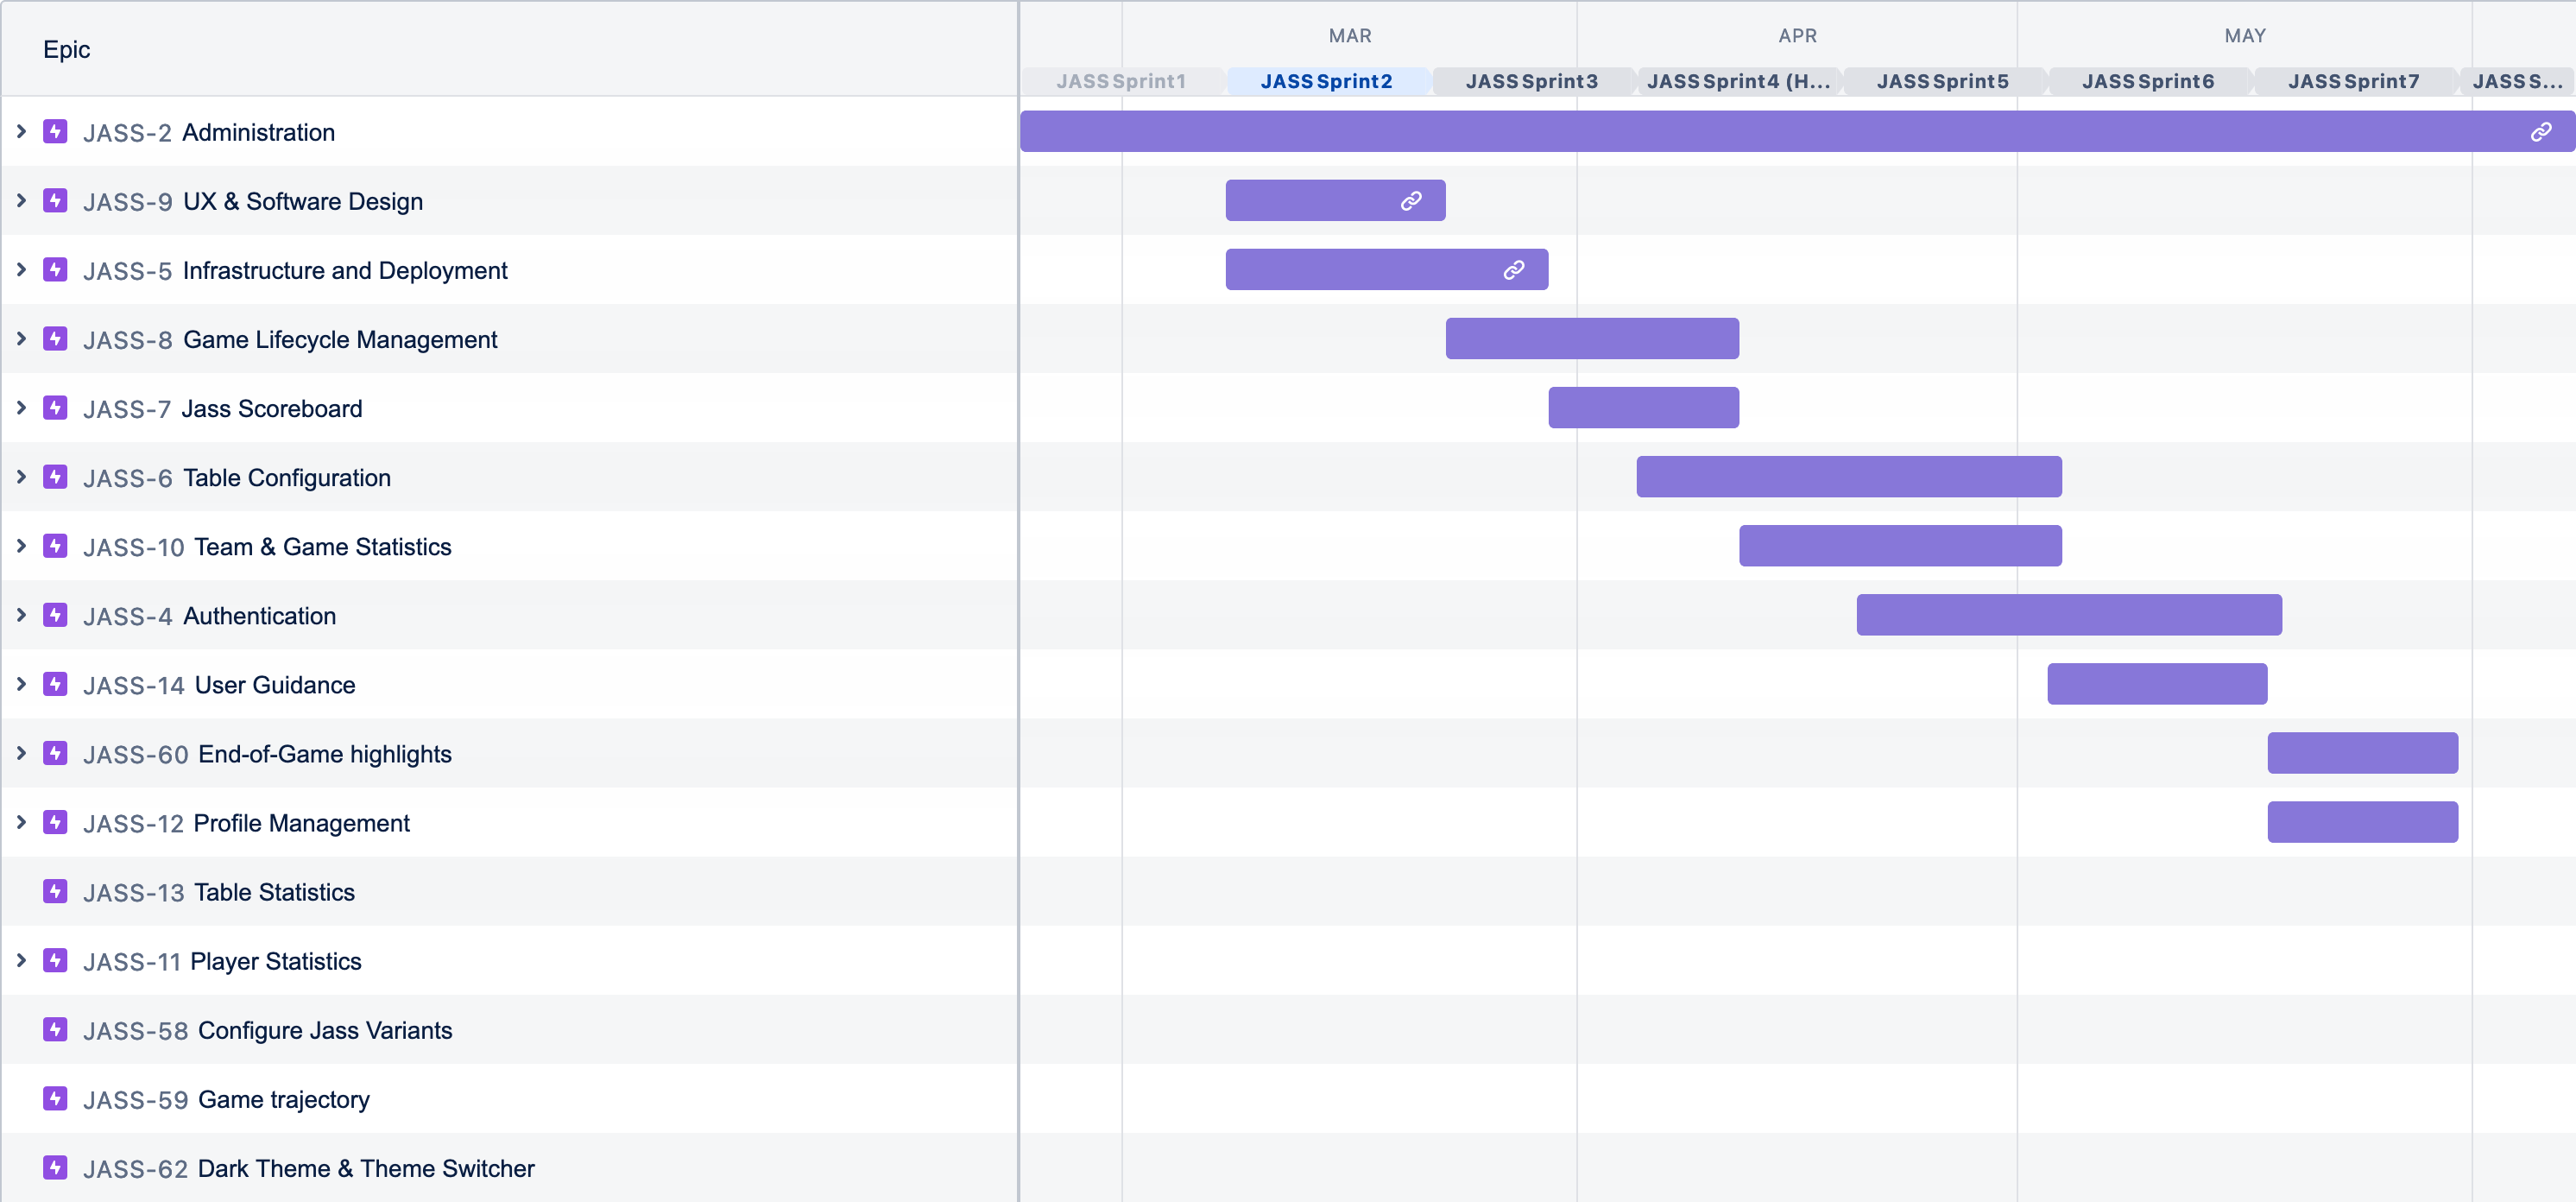
\includegraphics[width=\textwidth]{resources/jira-roadmap.png}
\chapter{Time Tracking Report}
\chapter{Personal Reports}

\instructions{
    Before the final submission, \textbf{personally reflect} your work in this project:
    
    \begin{itemize}
        \item What things did go well?
        \item Which areas could we improve?
        \item What were your personal highlights?
    \end{itemize}
    
    The information gathered in this chapter will be \textbf{\underline{very}} useful for all your future projects.
}
\chapter{Meeting Minutes}

\instructions{
    Add your meeting minutes here. As usual, try to keep them short and concise. 
}

\section{Kickoff Meeting 22.02.2022}

\subsection{Goals}
\begin{itemize}
    \item Choose tools (issue management, time tracking, VCS)
    \item Define and assign roles
    \item Rough long term plan
    \item Finalize vision of project
    \item Define and plan basic meetings
\end{itemize}

\subsection{Tools}

We plan on using GitLab for everything, including:

\begin{itemize}
    \item Version control system (Git monorepo)
    \item \href{https://gitlab.ost.ch/SEProj/GitLab_Time_Tracking_Tutorial}{Time tracking}
    \item Issue tracking
\end{itemize}

We use MS Teams for internal communication.

\subsection{Roles}

\begin{table}[H]
    \begin{tabular}{l|l}
    \textbf{Who} & \textbf{Roles} \\
    \hline
    Pascal & PO, DEV \\
    Marcel & DEVOPS \\
    David  & SM, DEV \\
    Jamie  & QA, DEV
    \end{tabular}
\end{table}

\subsection{Way of work}

We will likely use a combination of Scrum+RUP, but haven't decided yet. Will look into it next week.

\subsection{Vision Discussion}

After playing a "Jass" while using the existing Excel worksheet we found the following new features which might be implemented:

\begin{itemize}
    \item Disable input for teams which already played
    \item Add clock to see how long a player has been thinking (maybe not ideal because tracking a "Schiebe" is tedious)
\end{itemize}

\subsection{Long Term Plan}

Still not clear on how we plan to work, will be discussed next week.

\subsection{Meetings}

\begin{table}[H]
    \begin{tabular}{l|l|l}
    \textbf{Meeting} & \textbf{Schedule} & \textbf{Subject} \\
    \hline
    Weekly & Every Saturday & Progress and encountered problems \\
    Planning & Every other Saturday & Plan the next sprint, assign stories \\
    Retro & Every other Saturday & Review past spring, how to improve \\
    Review 1 & 07.03.2022 & Project Plan \\
    Review 2 & TODO & Requirements \\
    Review 3 & TODO & End of Elaboration \\
    Review 4 & TODO & Quality \\
    Review 5 & TODO & Architecture \\
    Project Presentation & TODO & TODO
    \end{tabular}
\end{table}

% TODO TimeTracking für dieses Meeting, 2h pro Person
\chapter{Usability Testing}\label{sec:uxTesting}

\section{Initial Usability Testing (Sprint 5)}

\subsection{Scope of testing}
For our first usability tests we defined the scope of the test on these 3 tasks:
\begin{itemize}
    \item Create a table
    \item Create a new game
    \item Enter round results
\end{itemize}

\subsection{Testers}
\begin{itemize}
    \item Daniel Maier
    \item Simon Link 
    \item Jeannette Vieser
    \item Michi Vieser
    \item Marc Honegger
\end{itemize}

\subsection{Methodology}
The testers were presented with our Test environment \url{https://jasstracker-test.honegger.dev/overview}.
Without giving any further instructions, we let the testers explore the application. 

\subsection{Test Results}
\begin{itemize}
    \item Create a table: unclear what a table is, creation easily done and understood
    \item Create new game: easily done and understood
    \item Enter round results: easily done and understood, however confirming the input is not possible with enter
\end{itemize}
Improvement suggestions: 
\begin{itemize}
    \item Numbering the games 
    \item Better visualization of timestamps
    \item Increase scoreboard size for better visibility
\end{itemize}


\section{Usability Testing Round 2 (Sprint 6)}

\subsection{Scope of testing}
For our second usability tests we defined the scope of the test on these 5 tasks:
\begin{itemize}
    \item Create a new Game (Updated UI Design)
    \item View Help Center
    \item Play as a Guest
    \item Register an Account
    \item Play a whole game
\end{itemize}

\subsection{Testers}
\begin{itemize}
    \item Nadia Bundi
    \item Daniel Maier
\end{itemize}

\subsection{Methodology}
The testers were presented with our Test environment \url{https://jasstracker-test.honegger.dev/overview}.
Without giving any further instructions, we let the testers explore the application. 

\subsection{Test Results}
\begin{itemize}
    \item Create a new Game (Updated UI Desing): new UI Design is easier to understand, concerning the teams
    \item View Help Center: Help Center is easy to find and informative
    \item Play as Guest: Playing as guest is harder to find, due to having to click on registration first
    \item Register an Account: easy to understand
    \item Play a whole game: having to explicitley complete a game seems unnecissary
\end{itemize}
Improvement suggestions: 
\begin{itemize}
    \item Total for one team, not per person
    \item Copy values from input to team colleagues scoreboard
    \item Being able to switch order of contracts (This is already an extension feature on our roadmap)
    \item Match is not 157 points but 257 points (This is also an extension feature on our roadmap)
\end{itemize}

\section{Final Usability Testing (Sprint 7)}

\subsection{Scope of testing}
For our final usability tests we defined the scope of the test on these 4 tasks and all previously mentioned tasks:
\begin{itemize}
    \item View Game Statistics
    \item View Profile Page
    \item View Player Statistics
    \item Play a whole game
\end{itemize}

\subsection{Testers}
\begin{itemize}
    \item Daniel Maier
    \item Kai Peter
    \item Anja Stöckli
    \item Anja Zahner
    \item Nadia Bundi
    \item Stefanie Hollenstein
\end{itemize}

\subsection{Methodology}
The testers were presented with our Test environment \url{https://jasstracker-test.honegger.dev/overview}.
The instructions given were to click on everything that they presumed was clickable and to report anything that didn't make sense to them. 

\subsection{Test Results}
\begin{itemize}
    \item View Game Statistics: some statistics were not clear at first glance of what they were representing, but with some consideration it made sense. It was also at first not clear that there were table statistics and specific game statistics
    \item View Profile Page: was easily understood and gave no questions
    \item View Player Statistics: easy to find and clear what is displayed 
    \item Play a whole Game:
    \subitem Create Table: It is unclear that the Table name is required, draggable fields are not intuitively understood
    \subitem Enter Scores: Works well with tab or mouse click, extension of entering negative values was not used unless help center was read through carefully beforehand
\end{itemize}
Improvement suggestions: 
\begin{itemize}
    \item Tisch erstellen as a button instead of the +
    \item Background should not be white on the table overview (to improve the first impression of the webapp)
    \item Completing a game should require a second confirmation like deleting a game
\end{itemize}

% Ensure all entries are printed, even if not referenced
\glsaddall
\printglossary
\newpage

\addcontentsline{toc}{chapter}{Bibliography}
\bibliographystyle{alpha}
\bibliography{bibliography}

\end{document}
